%Introduction
%\begin{savequote}[50mm]
%If our brains were simple enough for us to understand them, we'd be so simple that we couldn't.
%\qauthor{Ian Stewart }%The Collapse of Chaos: Discovering Simplicity in a Complex World
%\end{savequote}
%[Technologies for interoperable multi-device services]
\chapter{Adaptation methodology and model}
\chaptermark{Adaptation model}
\label{chap:adaptation}

\section{Overview}
New audiovisual experiences involve several contents through multiple Internet-connected devices. The TV is still the central hub of the living room, but it is often used simultaneously with other screens. Consequently, the user has the chance to enjoy different contents at once across multiple devices. However, no existing adaptation models are available to dynamically adapt such a multitude of contents to multi-device contexts. To address this gap, this chapter proposes a novel multi-device adaptation methodology to build adaptive user interfaces for multi-screen hybrid broadcast-broadband TV experiences that is extensible to any kind of content, device and user, and is applicable to different contexts considering technological evolution. 

The proposed methodology is the outcome of an extensive research arisen from a previous collaboration with broadcasters in the multi-device media service pilot described in Chapter \ref{chap:deployment}. This deployment has shown a set of lessons learned among which stands out the need of a usable user interface that guides the user across all the connected devices and bases its decisions on an efficient adaptation model built on top of the identification of the main user interface elements and design factors.

Additionally, preliminary evaluations have been performed to carry out the componentization of a broadcast service, make the typification of devices possible and study different aspects of the layouts shown in connected devices. These preliminary evaluations together with the previous deployment have guided the whole research towards the mentioned methodology. Taking all of this into account, the methodology provides a model which is formally described together with examples of its implementation. Finally, the methodology has been validated in terms of quality, efficiency and universality including all the results at the end of the chapter. 

\section{Overview of the adaptation methodology}\label{ov}

The aim of the adaptation process is to provide a suitable distribution of the contents of a hybrid broadcast-broadband programme into different devices' screens in the living room.
This content should be provided proactively and responsively, according to the context conditions and changes.

The proposed adaptation methodology aims to define a general multi-device adaptation model for hybrid broadcast-broadband services, such as the one deployed for the pilot experience described in Chapter \ref{chap:deployment}. However, instead of creating specific adaptation rules for each TV programme, they are made extensible for any kind of situation: any kind of TV programme or content, any device type, and any kind of UI layout template, to be used by any kind of user and in any context, and applicable even if technological changes occur (including new devices going further than AR/VR headsets or smart watches, new context conditions, new ways of interaction with TV or media, etc.).

This novel methodology identifies the elements, properties and criteria that should take part in the adaptation process \cite{Zorrilla2015} \cite{dominguez2017deployment} \cite{zorrilla2013} \cite{dominguez2018componentizing} \cite{dominguez2019methods}. 
More specifically, our approach is based on the definition of a general adaptation model that allows efficient implementations to be derived for the target multi-device broadcast environments. 
The effect of the context in the final user interface outcome is also considered. 
Figure \ref{fig:overview} shows an overview of the approach.

\begin{figure}	
	\begin{center}
		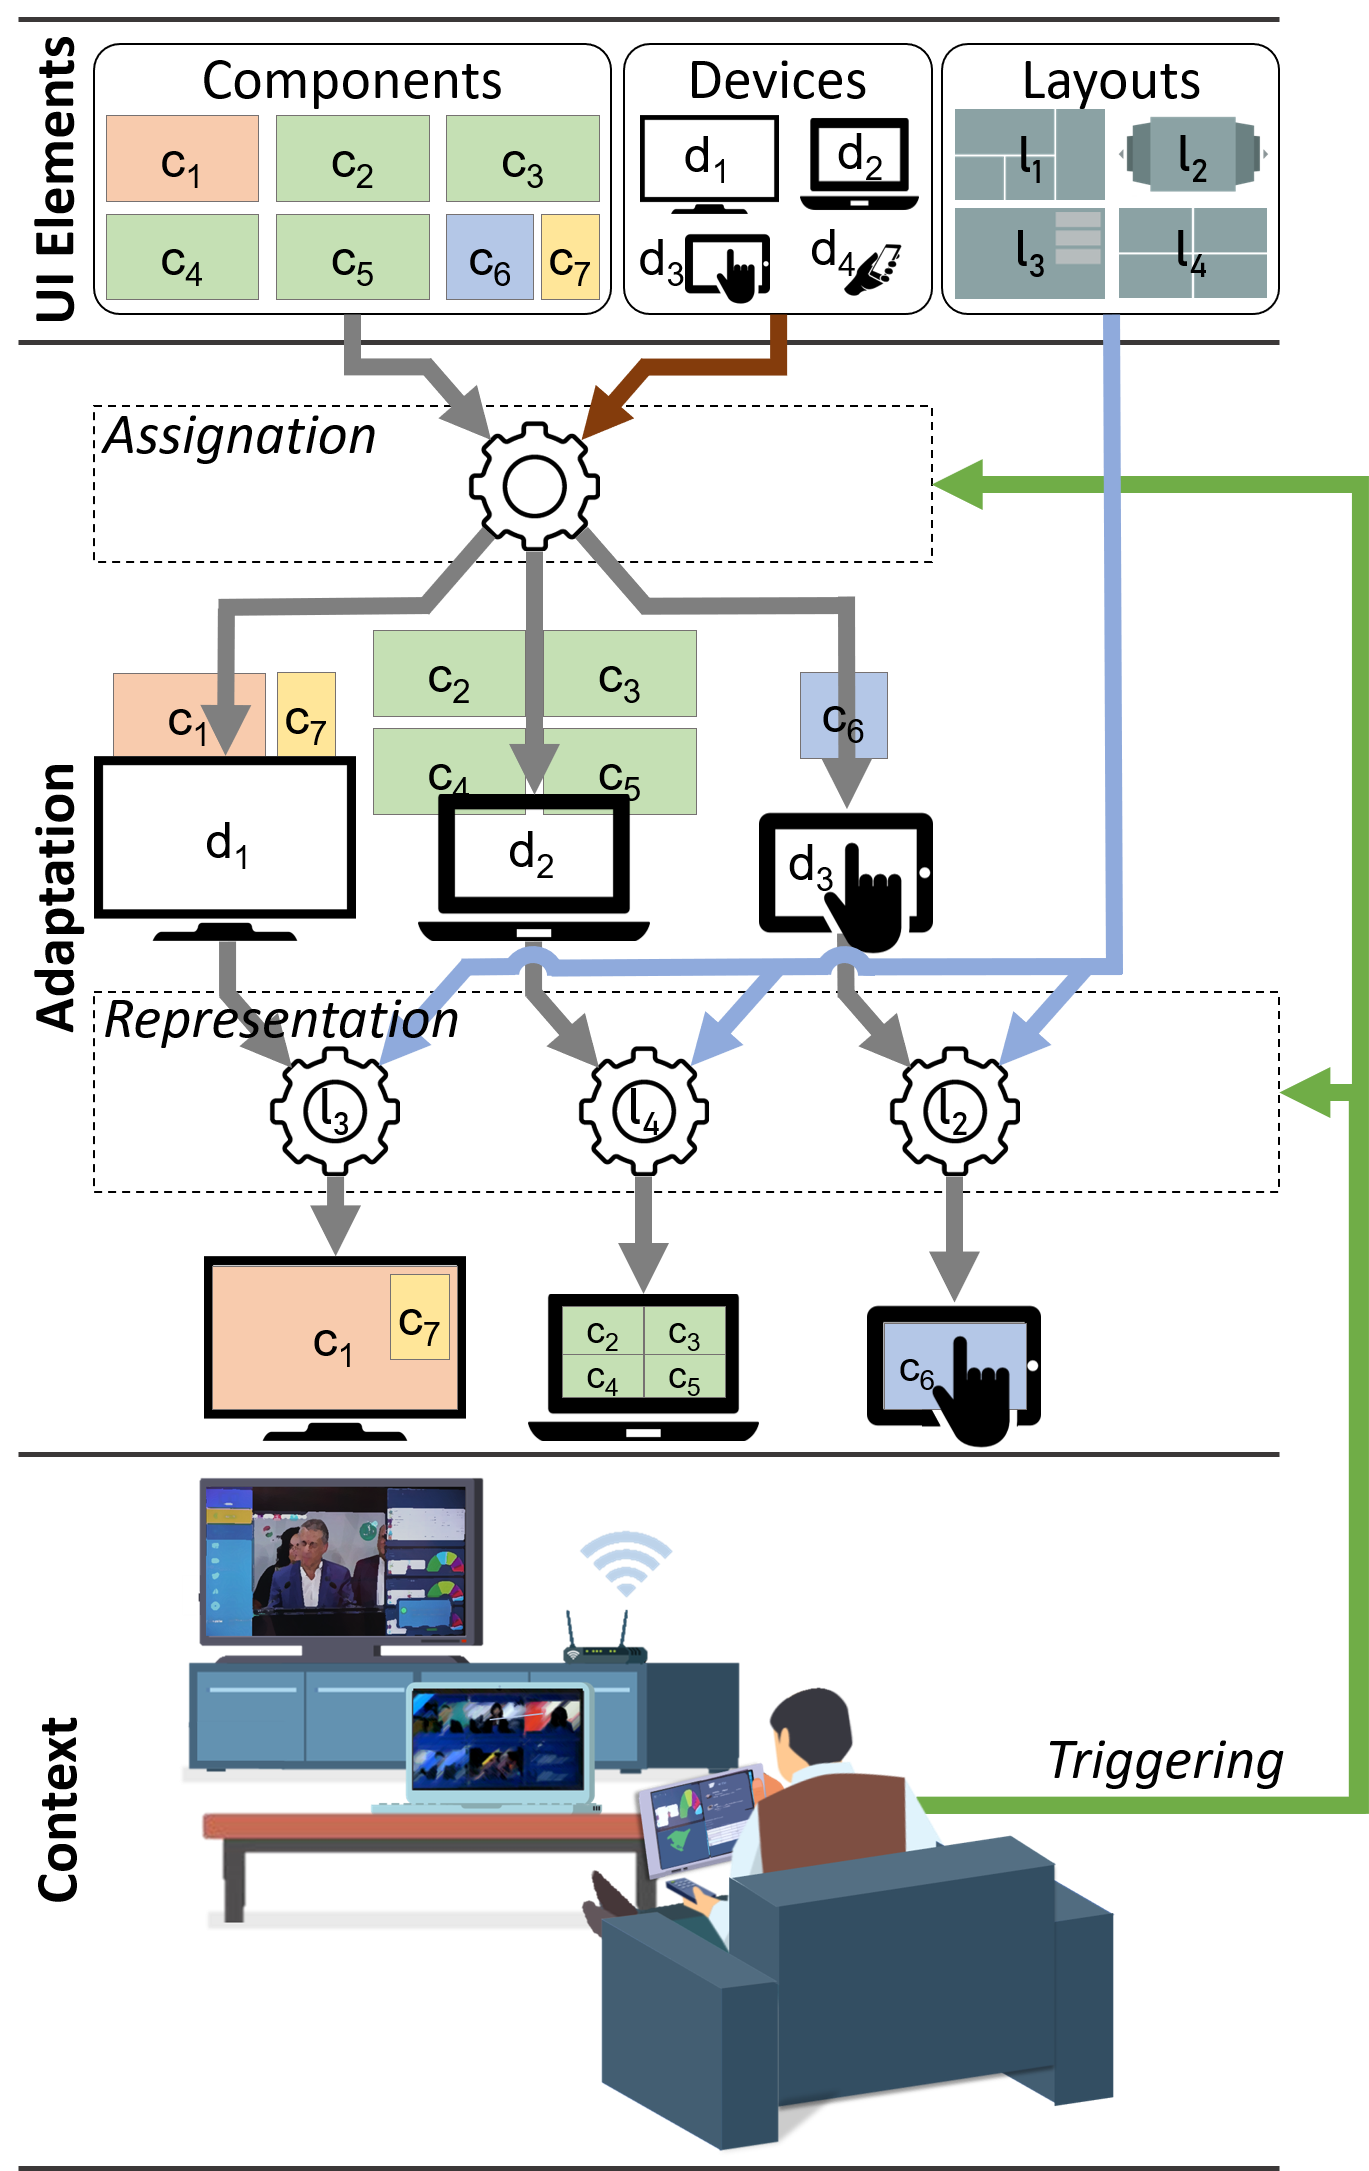
\includegraphics[width=0.6\textwidth]{overview.png}
		\caption{Overview of the proposed methodology}
		\label{fig:overview}
	\end{center}
\end{figure} 


In the following Sections, the adaptation model is described in detail, while a specific implementation of the model is presented in Section~\ref{imp}.
The adaptation model is described in three main parts:
\begin{enumerate}
	\item Identification and characterisation of the elements of the user interface (Section \ref{uie}).
	\item A flexible, modular, two-step characterisation of the adaptation process based on the aforementioned UI elements (Section \ref{ad}). 
	\item Finally, the role of the context as a drive of the adaptation process, which will be described on the basis of the implementation example
	%in the final result 
	(Section \ref{ctx}).
\end{enumerate}

To summarise, three types of elements of the user interface have been identified.
On one hand, a hybrid broadcast-broadband media service will have different pieces of content, such as the main programme (typically the broadcast), other media resources (multi-view live cameras, on-demand complementary content, etc.) and other types of information (statistics, graphics, banners, etc.). This work refers to all these elements related to the content as \textit{components}. On the other hand, the \textit{devices} that end-users will use to consume the content are also crucial elements to build an adaptive multi-device user interface. Finally, every screen taking part in the multi-device experience needs to visually organise the components in the display, assigning a location, size and aspect ratio to each of the components, creating user interface \textit{layouts}.

Regarding the adaptation strategy, the adaptation is divided into two goals:
\begin{enumerate}
	\item Maximising the quality of the distribution of the visual content components across the connected devices.
	\item Maximising the quality of the user interface layout in each device, given the components assigned to it.
\end{enumerate}

Then, the adaptation can be seen as being composed of two steps that are formalised as functions in the adaptation model, which we call \emph{assignation} and \emph{representation} respectively.

These two goals are interdependent regarding the general goal of maximising the adaptation process. 
However, we address the partial goals separately not only to have a clearer description of the adaptation model, but also to obtain a framework for efficient two-step implementations.

The rationale behind this divide-and-conquer strategy is the following: 
\begin{itemize}
	\item \textbf{Conceptual simplicity:} The adaptation problem is divided in two independent, well-defined sub-problems.
	\item \textbf{Performance:} As an optimisation problem, the computational complexity is dramatically reduced when the problem is divided, which is crucial in scenarios that include devices with limited computational resources. Furthermore, decoupling both goals in a two-step implementation allows for a more efficient distribution of processing in the second step.
	\item \textbf{Responsive answer to context changes:} The adaptation can be incremental, often involving the layout generation in just an individual device.
	\item \textbf{A suboptimal result might be preferable:} Finding an optimal solution requires addressing the adaptation problem as a whole. Nevertheless, responsiveness and low latencies are relevant requirements in a UI design, and optimality can be sacrificed if the obtained solution is reasonably good.
	\item \textbf{Previous experience:} The two-step adaptation was tested in the previous pilot deployment described in Chapter 3, with positive results. Additionally, broadcast professionals and researchers that were involved in the pilot can better contribute to the definition, implementation and validation of the defined model, overcoming the limitations of the pilot where specific adaptation rules need to be created.
\end{itemize}

Finally, regarding the context, the proposed approach is prepared to consider all possible circumstances that might influence the adaptation process. 
This context covers a full spectrum of situations, starting from the preferences and the interaction of end-users, environmental conditions, including lighting or acoustics, available connection bandwidth or processing capabilities, battery condition on mobile devices, the number of components that are being displayed on a device, etc. 
All of these context situations will feed the adaptation process and drive a new iteration when required.

The following sections formalise the definition of the main blocks proposed in the adaptation methodology.

\section{User interface elements}\label{uie}
To provide an adaptive multi-device user interface, it is important to identify the main elements, which are independent from the context and can be characterised or specified by the application developer: the content components, the target devices, and the  UI layouts.

\subsection{Content characterisation and componentisation} \label{components}
In recent years the trend of componentising the Web \cite{savage2015componentizing} has succeeded among most of the frameworks for Web applications development. 
``Web components'' \cite{webcomps} is an umbrella term for a handful of new specifications that give developers the primitives needed to build such interoperable, platform-level features. 
This componentisation, or modularisation of the content, allows for building a distributed system where each component can be easily moved from one device to another. 
Therefore, the entire content is divided into logic elements on top of the Web components standard, following the object-based broadcasting approach \cite{armstrong2014object}. 
Since a broadcast element (e.g., the main programme, an advertisement or a secondary video) is supported by a Web component, we will  refer to these broadcast elements as \emph{components}. 

The set of components for a specific hybrid broadcast-broadband programme can be formally defined as:
\begin{equation}
C = \{  c_1, c_2, ..., c_{N_C} \}
\end{equation}
For simplicity, we will also refer to a single component as $c$.

Each component could be characterised in terms of a set of properties \cite{bbcExp} \cite{sarkis2018multi}, such as:

\begin{itemize}
	\item \textbf{Attention}: The demand of attention required for that specific component regarding the entire multi-device media service, from the perspective of the content provider of the broadcaster. For example, the main programme is supposed to require high attention.
	\item \textbf{Interactivity}: The degree of interaction that the component allows depending on its type. For example, a chat component requires high interactivity.  
	\item \textbf{Processing Requirements}: The CPU/GPU processing and memory demands of a component (e.g. real-time decoding of H.264 and H.265 video streams). 
	\item \textbf{Broadcast Requirements}: The demand of a broadcast tuner to decode the TV content. 
	\item \textbf{Confidentiality}: The level of privacy required by a component, since it could include personal or customised information that might not be of interest for other viewers in the same physical space. This is the case, for example, of a secondary video, different from the main programme.
	%    \item \textbf{Geolocation necessity}: The demand of a GPS position to set up the content of a component
	\item \textbf{Geolocation necessity}: To allow for personalised, location aware setting of the content of a component.
	\item \textbf{Concentration}: The cognitive load demanded by the viewer to assimilate the information provided by a specific component. For example, concentration demand is higher for a social content than for an advertisement.
	\item \textbf{Source}: The creator of the component content, which is relevant, for example, to characterise the user generated content.
\end{itemize}

This set of properties could be extended to other properties depending on the use case, but we will consider them as stable and independent from the environment, and we will refer to them repeatedly. Nevertheless, for generalisation purposes, we define a set of formal properties:
\begin{equation}
P^{C} = \{ p_1, p_2, ..., p_{N_{P}} \}
\end{equation}
As we will see, the set of properties can be adapted in a flexible implementation.
For example, to describe a simple implementation where $N_P=3$, we will consider the properties $p_1$ = attention, $p_2$ = interactivity and $p_3$ = processing requirements.


For a given component $c$, a property vector $P^C[c]$ represents the values of each property, normalised in the range $[0, 1]$.
In our example, for a component $c$ (e.g., the main programme) the property vector could be:
\begin{equation}
P^{C}[c]=[1, 0, 0.2]
\end{equation}
which means that the component would fully require attention, would not require any interactivity and would present a low processing demand.
Note that for simplicity we are using the same notation for both the set of properties and the property vector.

All of the components in a service could be evaluated in terms of properties that would be quantified differently depending on the content type. 
To simplify the assignation of the property values to each of the components across the adaptation process, a classification of the components in \emph{component types} enables predefining a set of property values to each component depending on its type. 

In general, the set of component types is defined as $T^C$, 
and we consider a surjective function that maps each component onto a component type:
\begin{equation}
\mathcal{T^C}:C \to T^C
\end{equation}
Therefore we can, without loss of generality, associate the same property vector to every component of the same type: 
\begin{equation}
P^C[\mathcal{T^C}(c)] = P^C[c]
\end{equation}

An automatic typification of components is proposed and used in our implementation (see Section~\ref{imp}).

\subsection{Device characterisation} \label{devices}

Applications developed using Web technologies can be run on laptops, desktops, tablets, smartphones, smart TVs and even on consoles or other types of present or future devices. 
The only requirement is a Web browser and typically a connection to the Internet. 

Formally, the set of active devices in a given multi-device experience can be defined as follows:

\begin{equation}
D= \{  d_1, d_2, ..., d_{N_D} \}
\end{equation}

Again, there are a variety of properties that allow for differentiating one device from another and very useful to be considered during the adaptation process. 
For illustrative purposes, here an informal set of properties are defined that can be used to characterise current devices: 


\begin{itemize}
	\item \textbf{Screen Size}: The size of the display of the device. Trivially, the TV would have a large size and smartphones a small one. However, this property could integrate other features such as resolution or use distance. In this case it would then be better to consider the \emph{apparent size} of the screen device. 
	\item \textbf{Input Capabilities}: The features and mechanisms that a device provides for interaction. Current Connected TVs have low input capabilities, since all the interaction is through the remote control, while laptops, through the availability of keyboard and touchpad, have higher input capability.
	\item \textbf{Processing Capabilities}: The processing and memory capabilities of a device.
	\item \textbf{Graphic/video Capabilities}: The rendering and video decoding capabilities of a device. Note that current technologies use GPUs for both processing and graphic/video support.
	\item \textbf{Broadcast Capabilities}: The broadcast tuning and decoding capabilities of a device.
	\item \textbf{Privacy}: The level of privacy that a device provides in terms of enabling the ability to not share the content in the display with other viewers in the same physical space.
	\item \textbf{Mobility}: The degree to which a device can be in any location of the living room, which depends on factors such as the size/weight, the power supply or the need for an antenna. 
	\item \textbf{Geolocation capability}: The capability of a device to be auto-located, which can boost a personalisation of the contents.
	\item \textbf{Connectivity}: The level of network connectivity that a device is provided with, e.g., 3G/4G/5G, Bluetooth, WiFi, etc.
	\item \textbf{Environmental sensors availability}: The capability of a device to obtain physical or user context values such as the orientation or ambient luminosity. Note that a camera can be considered to be a generic sensor.
	\item \textbf{Aspect Ratio variability}: The set of different aspect ratios provided by the device. A TV provides a fixed aspect ratio, while smartphones and tablets can be turned 90\textdegree, providing a second aspect ratio.
\end{itemize}

To generalize, we define the set of device properties as:

\begin{equation}
P^D= \{ q_1, q_2, ..., q_{N_Q} \}
\end{equation}

For a given device $d$, a property vector represents the parametrisation of a device in terms of properties.
Again, considering a simple implementation where $N_D=3$ and $q_1=$ screen size, $q_2=$ input capabilities and $q_3=$ processing capabilities, a device $d$ (e.g. a Smart TV with a large display and limited interaction and processing capabilities) could be characterised as:
\begin{equation}
P^D[d]=[1, 0.2, 0.2]
\end{equation}

Characterising a device by its properties can be more easily performed using typification of the devices. For example, since most current devices can be classified into smartphones, tablets, laptops and Smart TVs, we could assign the same predefined properties values to all the devices of the same type. 
This means that, for instance, the screen size of all the smartphones could be characterised with the same value, which is much smaller than the value for the screen size of TVs.

Formally, we define the set of device types as $T^D$ and, similar to what it has been done for components, we consider a surjective function mapping each device to its device type: 
\begin{equation}
\mathcal{T^D}:D \to T^D  
\end{equation}
and thus, we can assign the same property vector to every device belonging to the same device type:

\begin{equation}
P^D[\mathcal{T^D}(d)] = P^D[d]
\end{equation}

As we will describe in Section~\ref{imp}, in a web multi-device environment such as the one we are considering, Web technology provides mechanisms that allow for an automatic typification of devices. 


\subsection{Layout characterisation}\label{layouts}

Today devices present a set of components to the user as efficiently as possible. 
The way those components are presented in the screen is called the layout. 
In terms of our adaptation model, a layout is a mapping of a subset of the set of components $C$ on the screen area of a device $d \in D$.

Formally, a set of possible layouts is defined as: 
\begin{equation}
L= \{  l_1, l_2, ..., l_{N_L} \}
\end{equation}

Each layout $l \in L$ can be defined in terms of a set of properties. 
Relevant layout properties are the following:

\begin{itemize}
	\item \textbf{Time sharing}: At a given time $t$, only a subset of $C_k$ is shown, thus each component is given a time slot of the screen resource.
	\item \textbf{Space sharing}: Components share the screen area, so a component should be reduced in size to fit a fraction of the screen.
	\item \textbf{Overlapping}: A component may overlap other components. 
	\item \textbf{Scrolling}: A component may shift smoothly, vertically or horizontally, across the screen. Note that when scrolling, the screen area is shared in both time and space. 
	\item \textbf{Distortion}: Components may be distorted to fit the assigned space of the screen both in scale and aspect ratio. If distortion is not provided, either the component should be cropped or an unused area is left.
	\item \textbf{Prioritisation of the components}: Components can be given different ranks, prioritising some over the others, which can be performed spatially (assigning more screen size) or temporally (assigning longer time slots). 
\end{itemize}

Moreover, a set of specific layout parameters are also relevant for a layout selection, including the minimum size of a component, maximum number of components to show at a time, etc. 
Note that these parameters are related to some device properties (e.g., screen size and resolution), component properties (e.g., attention) and user context (e.g., vision capabilities), among many others.

Again, to provide generalisation, we define a formal set of properties that characterises a layout: 
\begin{equation}
P^L = \{ r_1, r_2, ..., r_{N_R} \} 
\end{equation}

For a given number of components to show in a device, the variety of ways to organise them in the screen is very extensive. 
Even if temporal sharing is ignored, when searching for a layout solution to allocate $n$ components in $m$ possible locations, the number of possible layouts, $N_L$, is~\cite{sears1993layout}: 

\begin{equation} \label{combinatory2}
N_L = \binom{m}{n} n! = \frac{m!}{n!(m-n)!}n!
\end{equation}

Managing such a number of combinations can be prohibitive when using devices with limited computational resources, as is the case of our target environments. 
To cope with this problem, we will again use typification. 
Specifically, we generate a bounded set of layouts on the basis of a reduced collection of layout types or templates.
Examples of generic, well-known, user-accepted layout types or templates are Picture-in-Picture, Split  and Carousel. 
Note that a layout template can be characterised by the given set of layout properties.
A detailed description of the aforementioned templates, which we use in our implementations, will be provided in Section~\ref{imp}. 

In general, a layout template can be defined as a spatio-temporal scheme containing shapes that represent placeholders to be replaced by components at that location of the screen. 
The set of available layout templates is denoted as $T^L$ and a function maps the layouts onto layout templates:
\begin{equation}
\mathcal{T^L}:L \to T^L  
\end{equation}


\section{Adaptation Model}\label{ad}

Once the elements involved in the multi-device user interface adaptation are identified, an adaptation model can be presented. 
As mentioned in Section \ref{ov} our aim is to provide a flexible, modular adaptation model for which efficient two-step implementations are possible. 

In an adaptation process, the different properties of components, devices and layouts are combined to distribute the components among the connected devices in each moment, and, for each device, a layout for the assigned components is generated. 

Our proposal is based on the two partial goals defined in Section~\ref{ov}, which will be independently reached through the assignation and the representation steps.
Formally, the adaptation $\mathcal{H}$ can be defined as a composition of two component sub-functions \emph{assignation} (denoted $\mathcal{H}_1$) and \emph{representation} (denoted $\mathcal{H}_2$): 
\begin{equation}
\mathcal{H}=\mathcal{H}_1 \circ \mathcal{H}_2
\end{equation}

To properly define $\mathcal{H}_1$ and $\mathcal{H}_2$, in addition to the aforementioned primitive UI elements (i.e., components, devices and layouts) we introduce two new, intermediate elements.

The first of these elements is the \emph{assignment}. 
Let $A$ be the set of all possible combinations of the distribution of elements of $C$ on $D$. 
An assignment, $a \in A$, is represented as:

\begin{equation}
a = \{(d_1, C_1), (d_2, C_2), \ldots, (d_{N_D}, C_{N_D}) \}
\end{equation}
where $C_i \subseteq C$ represents a subset of the system components. As an example, the assignment shown in Figure~\ref{fig:overview} would be $\{(d_1, \{c1, c7\}), (d_2, \{c2, c3, c4, c5\}), (d_3, \{c6\})\}$. 

The second intermediate element is a set of layout $N_D$-tuples, denoted as $L^{N_D}$, which represent the layouts applied to every device in an assignment. 
Thus, a layout tuple $l^a \in L^{N_D}$ for an assignment would be:

\begin{equation}
l^a = (l_1, l_2, \ldots l_{N_D})
\end{equation}

On the basis of these elements, an adaptation function can be formally defined as:

\begin{equation}
\mathcal{H}:C \times D \times A \times L \to (A, L^{N_D}) 
\end{equation}

Regarding the assignation and representation functions, $\mathcal{H}_1$ makes use of the component and device set, $C$ and $D$, to produce an assignment:
\begin{equation} 
\mathcal{H}_1: C \times D \to A
\end{equation}
while $\mathcal{H}_2$ outputs a layout tuple to represent the elements of an assignment: 
\begin{equation}
\mathcal{H}_2: A \times L \to L^{N_D}
\end{equation}


In the following we will describe in more detail assignation and representation.


\subsection{Assignation} \label{s1}

The objective of the assignation is to define which component to show in which of the connected devices at each moment. 
For that, an assignation function is defined on the basis of the \emph{affinities} between devices and component types.

The affinity between a component and a device is defined in terms of the component and device properties. 
For each property pair $(p_i, q_j)$ an affinity value is assigned. 
For example, the component property \emph{attention} would have a high affinity with the \emph{screen size}, and a low affinity with the \emph{interaction capability} of the device. 
Instead, a high affinity should be defined between the component property \emph{interaction} and the device property \emph{interaction capability}.
For a given application environment, affinities can be established, e.g., upon usability tests. 

Affinity values are represented by an \emph{affinity matrix} $A_{f}=\{N_P \times N_Q\}$.
Then, the affinity of a component $c$ with a device $d$ could simply be calculated as the product of vector properties and the matrix $A_f$.
For notation convenience, we define an affinity function $\mathcal{A}$ that can be used to obtain the affinity of a component $c$ with a device $d$:

\begin{equation} \label{Eq:affinity}
\mathcal{A}(c,d) =P^C[c] \times A_{f} \times P^D[d]
\end{equation}
resulting in a scalar value that represents the affinity between component $c$ and device $d$.

As an example, consider three devices, \emph{tv}, \emph{smartphone} and \emph{laptop}, as candidates to hold a component (main programme, denoted $M$). 
We will consider three component properties: attention, interactivity and processing requirements, and three device  properties: screen size, input capabilities and processing capabilities.
We now estimate the requirements vector for $M$, i.e., the property values for this component, as:
\begin{equation} \label{Eq:PM}
P^C(M)=[1,0,0.2]
\end{equation}
which means that our main programme requires full attention and some processing (such as for rendering HD video), but it does not have any interaction requirements.
Additionally, we estimate the screen size, the input capabilities and the processing resources for each device:
\begin{equation} \label{Eq:PD}
\begin{split}
P^D[tv] & = [1, 0.2, 0.2] \\
P^D[smartphone] & = [0.2, 0.7,0.7] \\
P^D[laptop] & = [0.7, 1, 1]
\end{split}
\end{equation}
Finally, the affinity matrix could be the following:

\begin{equation}\label{Eq:AffEx}
A = 
\begin{bmatrix}
1 & 0.1 & 0.2 \\
0 & 0.6 & 0.1 \\
0.2 & 0.3 & 0.7 \\ 
\end{bmatrix}
\end{equation}

Note that the values chosen for the elements of A, although intuitive, are used only to provide an illustrative example.

To decide an assignment, the values from Eq.~\ref{Eq:PM}, \ref{Eq:PD}, \ref{Eq:AffEx} can be plugged into Eq.~\ref{Eq:affinity}, obtaining the following scalar affinity values:
\begin{equation} \label{eq:exampleassign}
\begin{split}
\mathcal{A}(M,tv) & = 1.14 \\
\mathcal{A}(M,smartphone) & = 0.558 \\
\mathcal{A}(M,laptop) & = 1.02
\end{split}
\end{equation}
which shows that the TV is the device with the highest affinity with the main programme component.

Despite the fact that $\mathcal{A}$ provides a simple order relation for the assignation function, in practice (as we will discuss in Section \ref{imp}) a multidimensional comparison could be preferable.
This comparison can be computed explicitly using the second multiplication of Eq. \ref{Eq:affinity}:

\begin{equation} \label{Eq:afproduct}
A_{f} \times P^D[d]
\end{equation}

This equation calculates, for each device, a vector whose elements can be directly mapped to the component's property vector. Following the example from before and applying Eq. \ref{Eq:afproduct}, we obtain the following values:

\begin{equation} \label{Eq:afproductExample}
\begin{split}
A_{f} \times P^D[tv] & = [1.06, 0.14, 0.4]  \\
A_{f} \times P^D[smartphone] & = [0.41, 0.49, 0.74] \\
A_{f} \times P^D[laptop] & = [0.8, 0.7, 1.1] 
\end{split}
\end{equation}

The affinity between a component and a device type can then be inspected visually, as shown in Fig. \ref{fig:reqgraph}. The plot shows the properties for the main component \emph{M} (in blue) and the vectors obtained from Eq. \ref{Eq:afproductExample}. From the figure it can be appreciated that in the example the TV appears to be the most suitable device for the main programme component, since differently to the other devices, the curve representing the TV (in red) contains the one representing the main programme requirements, $P^C(M)$ (in blue).
Using different values for the affinity matrix would have changed the shapes of the curves representing the different devices. 
By changing the affinity matrix depending on the use case, different criteria could then be applied to decide the best assignation. A more detailed example will be shown in Section \ref{imp}.

\begin{figure}
	\begin{center}
		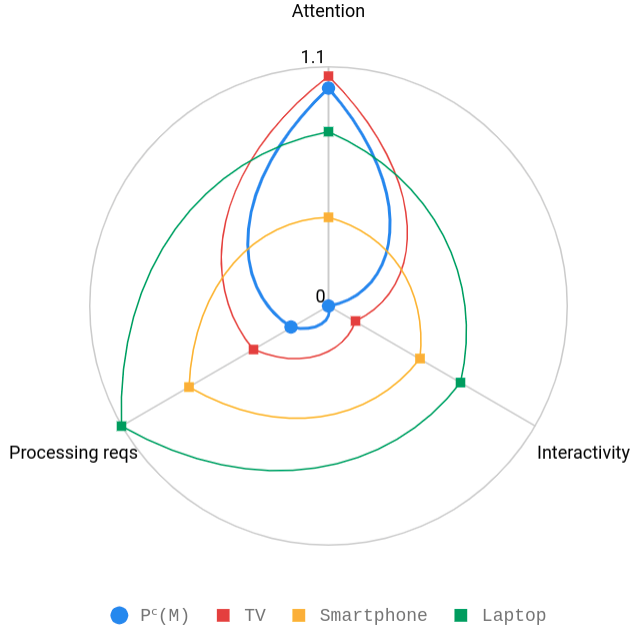
\includegraphics[width=0.55\textwidth]{chart.png}
		\caption{A visual representation of the affinity between component M and three device types.}
		\label{fig:reqgraph}
	\end{center}
\end{figure}

\subsection{Representation} \label{s2}

The objective now is to establish how components are organised in the devices' screens for a given assignment. 
Therefore, the representation function $\mathcal{H}_2$ will be applied for each device in $D$. 
In general, the problem of layout optimisation is NP-Hard \cite{drira2007facility} \cite{singh2006review}. 
To (partially) circumvent this complexity, in Section~\ref{layouts} we have introduced layout typification to consider a restricted set of layout templates. 
Nevertheless, a number of variables remain, mainly:
\begin{itemize}
	\item Layout template
	\item Component types
	\item Component properties
	\item Device type
	\item Device properties
	\item Number of components to be shown
	\item Criteria for the quality of the layout
\end{itemize}

Many other parameters could be added (aesthetics, user and physical context conditions...) which for simplicity are not considered here.  
Furthermore, the typification of components and devices will remove the component and device properties from the list. 

All these simplifications result in a model for layout generation that will be applicable in environments with limited devices and where responsiveness is a requirement.
The model of a layout generation includes the following elements:

\begin{itemize}
	\item a set of components $C_i \subset C$. 
	\item a device $d_i \in D$ of type $\mathcal{T^D}(d_i)$ where the layout is generated.
	\item a set of layout templates, $T^L=\{t_1, t_2, \ldots, t_{N_T}\}$.
	\item a set of layout quality (and efficiency) criteria, to be defined next.
\end{itemize}

From a formal perspective, our approach consists of defining a set of abstract quality criteria, $Z$, with associated quality expressions $\rho_k$ for all criterion $k$ in $Z$, and a general expression that combines all the quality expressions.
In section \ref{Imp-s2} we will describe the list of particular criteria used for evaluating the layout model.

The quality of a layout of $C_i$ on $d_i$ for a layout $l$ presents the following general expression:
\begin{equation} \label{Eq:layoutq}
\beta(l,d_i,C_i) = \prod_{k} \alpha_{k}^{w_k}
\end{equation}
where $w_k$ is an empirical coefficient that describes the relevance of criterion $k\in Z$ in the global quality of a layout, and $\alpha_k$ is the outcome of the specific function that evaluates the criterion $k$: 

\begin{equation}
\alpha_{k} = \rho_k (l,d_i,C_i) 
\end{equation}

The goal now is to determine the layout template that maximises the quality function. 
To simplify this, we will assume that for a given template $t \in T^L$ there is a layout $l^*$, such that $\mathcal{T^L}(l^*)=t$, which is optimal in $t$. 
In other words, we leave the task of finding, for a given template, the best possible layout of a set of components on a device to the implementation.
As we will show, this assumption is reasonable if the implemented quality criteria are based on simple geometric parameters, which are intuitive and usual.

Therefore, the problem of selecting a layout template for $C_i$ on $d_i$ can be formulated as:

\begin{equation} 
\label{eq:layout_max}
t_j:\max\limits_{j=1..N_{LT}} \beta(l^*_j,d_i,C_i)
\end{equation} 

As an example to illustrate layout selection in the model we are defining, we consider three layout templates: Carousel, PiP and Split. These templates are widely used in practice and are representative of both space- and time-sharing layouts.
In the absence of an extensive user evaluation, our previous experience \cite{Zorrilla2015}  \cite{dominguez2017deployment} suggests that there are some specific criteria that could make the user prefer one template over another, such as the rate of components shown on the screen, the ability to represent each component in its entirety or the efficiency in the use of the screen area. 

\begin{figure}
	\begin{center}
		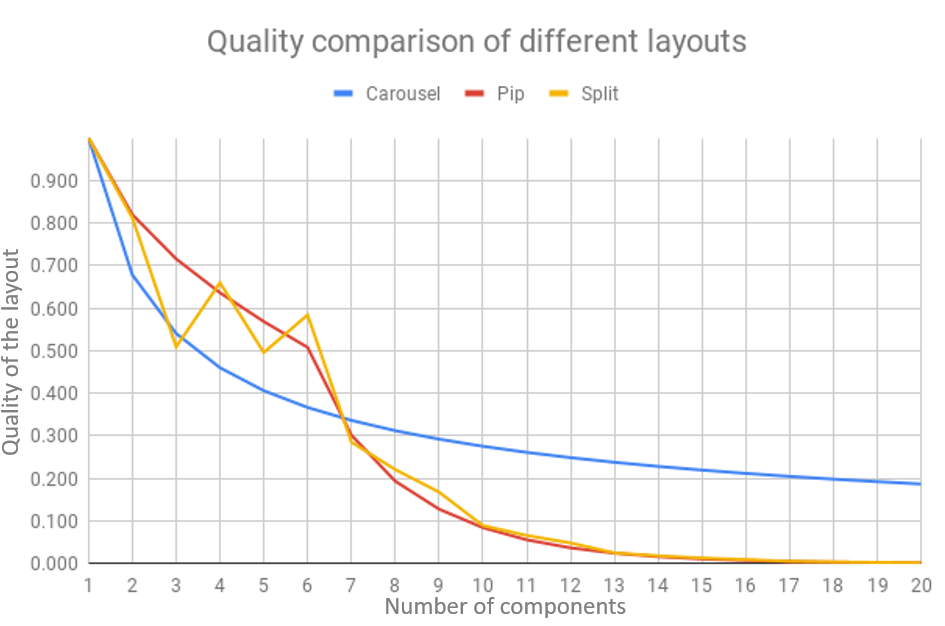
\includegraphics[width=0.8\textwidth]{QLayouts.png}
		\caption{Example of qualities comparison of different layouts for a laptop}
		\label{fig:Qlayouts}
	\end{center}
\end{figure}

As we will explain in detail in Section~\ref{imp}, we have used the aforementioned criteria to calculate the layouts qualities according to Eq.~\ref{Eq:layoutq}. 
Figure \ref{fig:Qlayouts} shows the resulting qualities of the three layout templates.
Eq.~\ref{eq:layout_max} will decide the best layout template depending on the number of components to be shown.
From the picture it is clear that, using the criteria above, PiP is the best layout for a low number of components, but it is surpassed by Split in cases where the number of components matches the number of cells provided by the Split template. 
Moreover, the Carousel layout is the best layout when there are more than 7 components to show on a laptop.


\section{Evaluation Model}

In this Section we present an evaluation model for the proposed two-step adaptation. In Section \ref{ov} we argued that the benefits of a two-step adaptation are at the cost of obtaining sub-optimal results.
This is inherent to the decoupling of the goal of the adaptation into two partial goals that are optimised separately and does not guarantee an optimal global adaptation solution.
This is because the optimal adaptation could result from an assignment not considered as the best in the assignation step, and thus is not evaluated in the representation step.

In order to set the quality of the solutions obtained by a two-step approach, we will consider the global optimal adaptation solution as a reference. 
Note that exploring all the solutions space in search of the global optimal solution may not be feasible as an implementation option for an adaptation method in a system with limited devices and real-time constrains such as ours.
In Section~\ref{val} we will provide a quantification of the computational costs to illustrate this. 

The approach for our evaluation model is based on ranking the two-step results in relation to the global optimal solutions, according to a quality metric.
This metric is computed as the mean of the individual quality of the adaptation for every  component in $C$. 
Note that the metric involves two criteria that match with the defined partial adaptation goals:
\begin{enumerate}
	\item The quality of the assignment of the component, i.e., the affinity of the component with the assigned device.
	\item The quality of the representation of the component on the assigned device screen for the layout selected.
\end{enumerate}

Let $\mathcal{E}$ be a function that evaluates the quality of the adaptation for a single component $c \in C$ given an assignment $a=\{(d_1,C_1), (d_2,C_2), \ldots, (d_{N_D},C_{N_D})\}$. 
Let $l_i\in L^a$ be the layout applied to element $a_i=(d_i,C_i)$ in $a$. 
We evaluate the overall adaptation quality of $c$ as the product of the assignment quality and the representation quality.
In general:

\begin{equation} \label{Eq:E}
\mathcal{E}(c,a_i) = \mathcal{E}_1(c,d_i) \cdot \mathcal{E}_2(c,a_i,l_i)
\end{equation} 

The point now is to provide an estimate for both $\mathcal{E}_1$ and $\mathcal{E}_2$.

\subsection{Evaluating component assignment}

In Section~\ref{s1} we argued about the multi-objective nature of the assignment problem. 
Since comparing multi-dimensional figures is cumbersome, for our evaluation model we apply the scalar expression of the affinity calculated by function $\mathcal{A}$ according to Eq.~\ref{Eq:affinity}.
Note that this is a worst-case estimate for the real assignment performed by the assignation step, since introducing constrains in the assignment, as represented in the example of Figure~\ref{fig:reqgraph}, could prevent choosing the best ranked assignment according to Eq.~\ref{Eq:affinity}.

In summary, 

\begin{equation} \label{Eq:E1}
\mathcal{E}_1(c,d_i)= \begin{cases}
\mathcal{A}(c,d_i) & \text{if $c \in C_i$} \\
0 & \text{otherwise}
\end{cases}
\end{equation}


\subsection{Evaluating component representation}

Eq.~\ref{Eq:layoutq} defines a function $\beta$ that outputs the quality of the representation of an assignment $a_i=(d_i,C_i)$ using a layout $l_i$. 
As we have shown in Section~\ref{s2}, quality is measured in terms of the set of criteria on the basis of geometric parameters. 
Because for a layout the entire set of components $C_i$ should be considered, to obtain an estimation of the quality of the representation of an individual component $c \in C_i$, we will take Eq.~\ref{Eq:layoutq}  and assume that every component in $C_i$ has the same impact on the quality of the representation of $C_i$, i.e.:

\begin{equation} \label{Eq:E2}
\mathcal{E}_2(c,a_i,l_i)= \frac{\beta(l^*_i,d_i,C_i)}{\mid C_i \mid}
\end{equation} 

\subsection{Calculating the overall quality}

Combining Eq.~\ref{Eq:E}, \ref{Eq:E1}, and \ref{Eq:E2}, we determine that the quality of adaptation of a component $c \in C$ for an assignment $a_i=(d_i,C_i)$ to be represented by a layout $l_i$ results in the following:

\begin{equation} \label{Eq:E-Overall}
\mathcal{E}(c,a_i) = \begin{cases}
\frac{\mathcal{A}(c,d_i) \beta(l^*_i,d_i,C_i)} {\mid C_i \mid} & \text{if $c \in C_i$} \\
0 & \text{otherwise}
\end{cases}
\end{equation} 

Eq.~\ref{Eq:E-Overall} can be applied to every component $c \in C$ for any adaptation solution, i.e., whatever combination of assignments and possible layouts. 
The overall quality of an adaptation $\mathcal{H}=(C,D,a,L^a)$ can be estimated by the addition of the individual estimations calculated by Eq.~\ref{Eq:E-Overall}. 
The resulting expression is:

\begin{equation} \label{Eq:E-All}
\mathcal{E}^{\mathcal{H}}(C,D,a, L^a) = \frac{1}{N_D} \sum_{i=1}^{N_D}\Big[\frac{\beta(l^*_i,d_i,C_i)}{\mid C_i \mid} \sum_{\forall c \in C_i} \mathcal{A}(c,d_i)\Big]
\end{equation} 

Observe that, for simplicity, in Eq.~\ref{Eq:E-All} we are assuming that $c \in a_i$.


\section{Implementation}\label{imp}

In Section~\ref{uie} and Section~\ref{ad} we described a model for multi-device adaptation in hybrid broadcast. 
The model is aimed at being general enough to allow for specific implementations, including particular sets of components, current and forthcoming devices, or alternative layout templates. 
On the other hand, the outputs in the adaptation strongly depend on a set of parameter values that should be configured upon the use of the system in a real deployment, either by manual setting or by an automatic learning process.

The aim of this section is to provide a comprehensive description of how an implementation can be derived from the model. 

For this, we describe an implementation of the model based on a set of categorised components, devices and layouts that we consider as representative and reasonably complete for current hybrid broadcast broadband services.

Furthermore, a reduced subset of the defined element properties has been implemented for this prototype, which can be easily extended as we will show in Section~\ref{val}.
As already mentioned in Section \ref{s1}, the parameters have been chosen to intuitively make sense. Obtaining them using a machine learning approach or by conducting a user evaluation, although it would be convenient when deploying a real application, is outside the scope of this research. 
As described in Section~\ref{ov}, for efficiency reasons, we apply our adaptation model to follow a two-step implementation. 
Step~1 is in charge of selecting an optimal assignment of components to devices in terms of affinity criteria.
Step~2 is executed in each device to find an optimal layout for the assignment of components to the device. 
Note again that in Step~2, the layouts evaluation is conditioned by the previous assignment decision in Step~1, hence a global optimal adaptation solution could not be reached by this two-step approach. 
Instead, a reasonably good solution is acceptable for our purposes, while the two-step approach brings better responsiveness and less energy consumption.
Furthermore, considering the dynamic behaviour of a multi-device context, the system could apply small corrections whenever the context changes, providing  agile, incremental assignations.

In the remainder of this section, the specific component and device types considered are described, as well as the layout templates used. For that, the carried out preliminary evaluations are also described which have prompted the considered element types.
Then, the implementations for Step~1 and Step~2 of the adaptation process are described regarding the specific scenarios considered, the solutions provided, and trade-offs taken.
Finally, a mechanism for triggering the adaptation process is described with the aim of preserving an acceptable adaptation quality upon context changes. 

\subsection{Component types and properties} \label{imp_comp}

Nowadays, several content types can be found on TV programmes and Internet. In order to be able to distribute them intelligently across the different devices used simultaneously in a multi-device experience, a componentization and a typification is needed. In order to do that, a componentization of traditional TV programmes which are candidates of becoming multi-device TV programmes was carried out.

\subsubsection{Componentization of a TV programme}
We conducted a research~\cite{dominguez2018componentizing} to provide component typification. The work proposes a way of componentising hybrid broadcast-Internet media services, based on a methodology that analyses the contents of different TV programmes and groups them in terms of the component properties we have defined in Section~\ref{components}. Next subsections provide the methodology followed as well as the componentization results.

 
\paragraph{Methodology}
The criteria to select the broadcast emissions to be analysed was to bound the amount of emissions to those that are watched by the highest audience volume. That way, the contents obtained as a result were contents that the audience is used to find at present, having the least impact on the experience and contributing to the usability of the final adaptation model. Taking this into account, the selection of the emissions was done as follows:

\begin{enumerate}
	\item \textbf{Selection of the 5 countries in European Union with the highest population}, being Germany, France, United Kingdom, Italy and Spain the countries fulfilling that condition. 
	\item \textbf{Selection of the most viewed TV channel from each one of the previous countries.} \cite{staGermany}, \cite{staFrance}, \cite{staUk}, \cite{staItaly} and \cite{staSpain} show that ZDF, TF1, BBC, RAI 1 and Telecinco were the most watched channels in each country in 2016. 
	\item \textbf{Selection of the most appropriate programmes to promote social interaction}. Some programmes are more suitable for interactive experiences \cite{geerts2008implications} due to the large amount of content they show or the motivation they generate for the user to share his experience in social networks. From a list of 18 programme genres based on the EBU \cite{ebu} classification, the most suitable genres to promote a social interaction are: News, soap, quiz, sports, reality show and talk show. The suitability is evaluated depending on how much people talk and share during and after the TV show. All of them were initially considered but soap and reality show were finally discarded since soap are not designed to be componentized and reality shows are focused on other type of social interaction, different from what we are looking for. Therefore, the four programme types that were analysed could be described as follows:
	\begin{itemize}
		\item \textbf{News:} Daily scheduled programme that reports current events. News is reported as a series of individual stories and can include a variety of contents. 
		\item \textbf{Quiz:} Programme in which a single or a group of contestants compete in answering questions.
		\item \textbf{Sports:} Programme in which a sport competition is broadcasted, preferably live.
		\item \textbf{Talk show:} Programme in which a panel of guests discuss various topics such as politics, celebrities personal life or news summaries. 
	\end{itemize}
	\item \textbf{Selection of one emission per programme for each type and country.} One emmission per programme was considered to be enough since all emissions of the same programme followed more or less the same structure. Emissions from 2016 or 2017 were searched online in order to ensure contemporary content. 
	\item \textbf{Selection of the first 30 min from each emission}, which experimentally was verified to be enough to identify the type of elements that could appear on it.
	\item \textbf{Check the impact of advertisements} in both public and private channels. The previous programmes selection included both public and private channels, which would allow to detect the mentioned impact.    
\end{enumerate} 

Table \ref{tab:selEmissions} shows the summary of the analysed emissions per country, channel and programme type. 

\begin{table}[ht]
	\begin{center}
		\caption{Summary of the selected emissions}
		\label{tab:selEmissions}
		\begin{tabular}{||c|c|c|c||}
			\hline
			\textbf{Country} & \textbf{Channel} & \textbf{Type} & \textbf{Programme} \\
			\hline
			\multirow{4}{*}{Germany}   & \multirow{4}{*}{ZDF}   & News             & Heute journal \\ 
			&  & Quiz & Der quiz champion \\
			&  & Sports & Ski \\
			&  & Talk show & Heute show \\
			\hline
			\multirow{4}{*}{France}    & \multirow{4}{*}{TF1}              & News             & Le journal de 13h  \\ 
			&  & Quiz & Money drop \\
			&  & Sports & Football \\
			&  & Talk show & 24 heures en question \\
			\hline
			\multirow{4}{*}{UK}        & \multirow{4}{*}{BBC}              & News             & News at 10  \\ 
			&  & Quiz & Impossible\\
			&  & Sports & Golf \\
			&  & Talk show & Sundays politics \\
			\hline
			\multirow{4}{*}{Italy}     & \multirow{4}{*}{RAI1}             & News             & Telegiornale TG1  \\ 
			&  & Quiz & L'eredità \\
			&  & Sports & Cycling \\
			&  & Talk show & Agorà \\
			\hline
			\multirow{4}{*}{Spain}     & \multirow{4}{*}{Telecinco}        & News             & Informativos Telecinco  \\ 
			&  & Quiz & Pasapalabra \\
			&  & Sports & MotoGP \\
			&  & Talk show & El programa de Ana Rosa  \\
			\hline
		\end{tabular}
	\end{center}
\end{table}

\paragraph{Resulting component types}

As a result large list of different elements were identified for each programme type. All of those elements are included in Table \ref{tab:elemlist} in an extensive way and the most representative can be found in Figure \ref{fig:examples}. As can be seen, the four type of programmes show a variety of elements along the emission. Pictures 1 to 4 in Figure \ref{fig:examples} show different video signals for live connections, participant cameras or videos sent by the users while Pictures 5 to 12 in  Figure \ref{fig:examples} show other elements appearing along the emission such as advertisements, headlines, text, data, questions, classifications, or twitter content. Some of these elements in Table \ref{tab:elemlist} and Figure \ref{fig:examples} exhibit certain degree of similarities that suggest the componentization of a TV programme.



\begin{figure}	
	\begin{center}
		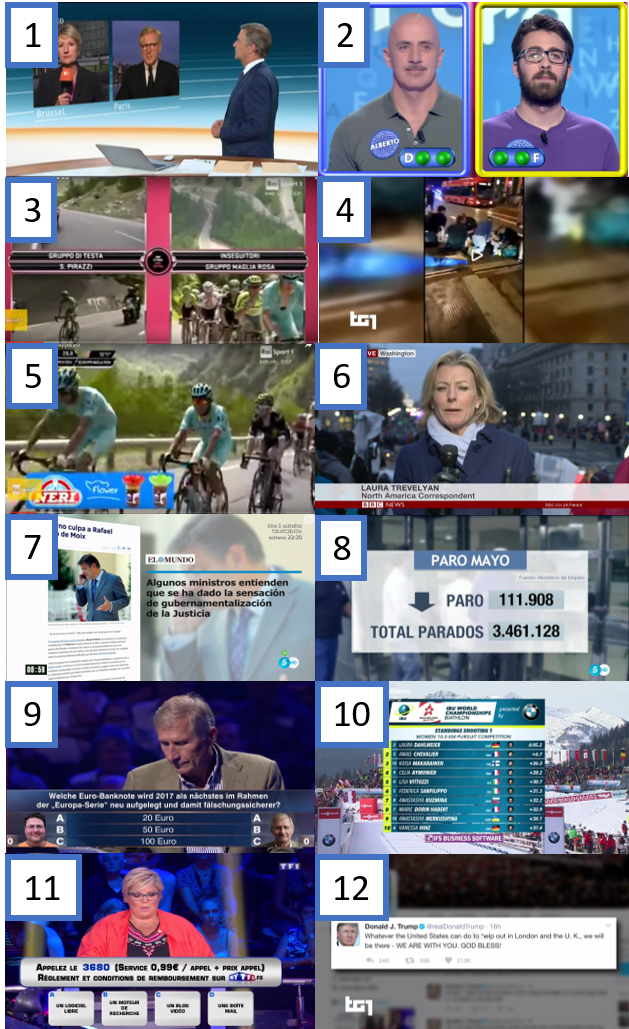
\includegraphics[width=0.5\textwidth]{all}
		\caption{Examples of different elements found in the analysed emissions}
		\label{fig:examples}
	\end{center}
\end{figure} 


\begin{table} 
	\caption {Summary of the identified elements in the analysed emissions}\label{tab:elemlist}
	\begin{tabular}{||L|L|L|L||}
		\hline
		\textbf{News} & \textbf{Quiz} & \textbf{Sports} & \textbf{Talk show} \\
		\hline   
		\begin{itemize}[leftmargin=.1in]
			\setlength{\itemsep}{-0.3\baselineskip}
			\item Main video signal
			\item Live connection 
			\item Pre-recorded videos 
			\item Interviews 
			\item UGC 
			\item Programme name 
			\item Presenter name 
			\item Journalist name 
			\item Name of the interviewed person 
			\item Headlines 
			\item Live, place 
			\item On-screen graphic 
			\item Weather   
			\item Maps
			\item Statistics
			\item Text       
			\item Twitter content (A tweet overlapping a Twitter page)
			
		\end{itemize}
		& 	
		\begin{itemize}[leftmargin=.1in]
			\setlength{\itemsep}{-0.3\baselineskip}
			\item Main video signal
			\item More than one contestant at the same time 
			\item Contestant presentation video 
			\item Contestant info: name, job, place 
			\item Time
			\item Attempts 
			\item Scoreboard 
			\item On-screen graphic 
			\item Questions (different subjects, musical, fill in the gap, photos, etc)
			\item Answers (true/false, 4 options, fill in the gap)    
			\item Info for the casting     
			\item Prizes (for the contestant, for the audience) 
			\item Audience participation (answer by sms, hashtags to follow)  
			\item Adverts (other programmes, first releases)
		\end{itemize}
		& 	
		\begin{itemize}[leftmargin=.1in]
			\setlength{\itemsep}{-0.3\baselineskip}
			\item Main video signal
			\item Different angles, athletes or race points, on board, etc
			\item Interviews
			\item Replays: plays, overtakes, laps, etc 
			\item On-screen graphic
			\item Small detail classifications (fastest lap, distances, scoreboard, starting line)
			\item Extended classifications
			\item Tournament info
			\item Schedule
			\item Circuit, stage information: name, curves, kms, records, mountains, etc
			\item Athletes, coach, teams info
			\item Weather
			\item Previous results
			\item Performance info(speed, distance, time) 
			\item Audience participation (raffles by call or sms, hashtags to follow, WebSite)
			\item Adverts (products, brands)
		\end{itemize}
		& 	
		\begin{itemize}[leftmargin=.1in]
			\setlength{\itemsep}{-0.3\baselineskip}
			\item Main video signal
			\item News 
			\item Interviews 
			\item Live connections 
			\item Debate participants 
			\item UGC 
			\item On-screen graphic 
			\item Headlines 
			\item Name of the person talking 
			\item Info of the person talking 
			\item Breaking news 
			\item Time        
			\item Politician’s cites
			\item Newspapers headlines
			\item Statistics
			\item Graphs
			\item Text
			\item Audience participation (hastags to follow, answers by call or sms, answers by Facebook or Twitter)
			\item Adverts (other programmes)
		\end{itemize} \\
	\hline
	\end{tabular}
\end{table}

Following this criteria, 8 components types were identified to be used when the TV programme evolves into an interactive multi-device TV show:
\begin{enumerate}
	\item \textbf{Main programme}: The mainstream audiovisual content that drives the experience.
	\item \textbf{Advertisements}: Business-related resources advertising something within the TV programme. 
	\item \textbf{Secondary videos}: Additional videos sourced by the broadcaster. 
	\item \textbf{Banners}: Additional information including notifications, headlines and small texts.
	\item \textbf{Static Data}: Elements that show relevant data, longer-texts or images, that might not bring interaction by the user.
	\item \textbf{Interactive Data}: Elements that show relevant data, diagrams or tables that might bring interaction by the user.
	\item \textbf{UGC - User Generated Content}: Additional videos generated by the viewers.
	\item \textbf{Social content}: Additional information coming from the opinion of the viewers (social networks, a quiz, etc.).
\end{enumerate}

An example implementation of our model can be based on this set of component types, or a subset of it. 
Every component $c \in C$ in the multi-device experience is labelled with one of the aforementioned types, which provides a straightforward implementation of function $\mathcal{T^C}$.
Then, assigning property values to $c$ can be systematically made from predefined values that are mapped to component types.
For a simple prototype implementation, we will use three of the component properties defined in Section~\ref{components}: attention, interactivity and processing requirements, following the example initiated in Section~\ref{s1}.

\subsection{Device types and properties} \label{imp_dev}

In the context of hybrid broadcast-Internet media services, such as the one described in Chapter \ref{chap:deployment}, there are usually four types of devices involved, also called \textit{core devices} or \textit{core screens} \cite{nagel2015multiscreen}. 
We are talking about smartphones, laptops, tablets and Smart TVs.
These devices will be the basis for our implementation, even though the model we have defined is able to incorporate other types of devices, such as smartwatches, VR/AR headsets or future incoming HCI devices.

Device properties will be generically assigned to the considered device types. 
Most of the properties can be theoretically obtained from the scripting capabilities of Web browsers, frameworks or libraries. 
However, this is sometimes not possible and often provides false positives, making such information unreliable. 
Finally, device typification must be performed at run-time. 

In this context, we conducted a research in which we used the information about the device made available by the browser to implement device typification. 
The work \cite{dominguez2019methods} analyses the existing tools for Web-based device type detection. It also compares three different methods for automatic device type detection using the User Agent of the browser and basing their knowledge on different learning systems and statistical models. And finally, it provides an empirical comparison of the selected methods.

\subsubsection{Analysis of existing tools for Web-based device type detection}\label{soa}

There are numerous open source and proprietary libraries or scripts that detect specific features and the type of devices. Most of these tools compare the User Agent against a database or a token list of specific terms and return a device type. A User Agent is a string identifying the browser and operating system to the web server. Table \ref{tab:uaex} shows an example of User Agent for each device type. As can be seen, the contents of the User Agent field vary from browser to browser and although it contains tokens which provide valuable information about the browser and device, a standardised User Agent format does not exist. Moreover, as the number of Web-enabled devices increases, the variety of different User Agent strings grows.

\begin{table}
	\centering
	\caption{Examples of User Agent strings}
	\label{tab:uaex}
	\begin{tabular}{||c|p{10cm}||}
		\hline
		\textbf{Device type}&\textbf{User Agent example} \\
		\hline
		Mobile & "Mozilla/5.0 (Linux; Android 7.1.1; Moto G (5S) Plus Build/NPSS26.116-64-8) AppleWebKit/537.36 (KHTML, like Gecko) Chrome/66.0.3359.126 Mobile Safari/537.36"
		\\
		\hline
		Tablet & "Mozilla/5.0 (Linux; U; Android 2.2; en-gb; GT-P1000 Build/FROYO) AppleWebKit/533.1 (KHTML, like Gecko) Version/4.0 Mobile Safari/533.1"\\
		\hline
		Desktop & "Mozilla/5.0 (X11; Linux x86\_64) AppleWebKit/537.36 (KHTML, like Gecko) Chrome/71.0.3578.98 Safari/537.36"\\
		\hline
		TV & "Mozilla/5.0 (Linux; Tizen 2.3; SmartHub; SMART-TV; SmartTV; U; Maple2012) AppleWebKit/538.1+ (KHTML, like Gecko) TV Safari/538.1+" \\
		\hline		
	\end{tabular}
\end{table}

Since none of the existing libraries provide details about their accuracy retrieving device features, a dataset \cite{uagit} of 3228 User Agent strings was assembled and for each library described in \cite{dominguez2019methods} it was computed the accuracy in detecting the device type. The User Agent strings in the dataset were categorized into four classes: \emph{desktop}, \emph{mobile}, \emph{tablet} or \emph{TV}. The distribution of the devices in the dataset is shown in Table \ref{tab:indist}, while the results of the evaluation are available in Table \ref{tab:soaAcc}. The value N/A was used in the table in case the library did not detect that particular class of devices. The best results were achieved by Categorizer.js (a deprecated library) with an accuracy of 91.8\% while Detectizr.js was the library with the worst performance since it detected the device type correctly only 31.8\% of the times. 

Methods as the aforementioned require updated databases and token lists for identifying correctly new devices, which is a very high maintenance task doomed to fail at some point in the future. Consequently, more efficient and advanced methods, which require less upkeep, are needed.


\begin{table}
	\centering
	\caption{Independent dataset distribution by device type}
	\label{tab:indist}
	\begin{tabular}{||c|c||}
		\hline
		\textbf{Device type}&\textbf{Number of UA in dataset} \\
		\hline
		Mobile & 1000\\
		Tablet & 1000\\
		Desktop & 1000\\
		TV & 228 \\
		\hline
		Total & 3228\\
		\hline
	\end{tabular}
\end{table}

\begin{table}
	\centering
	\caption{Accuracy of existing device type detection libraries}
	\label{tab:soaAcc}
	\begin{tabular}{||c|c|c|c||}
		\hline
		\textbf{Method}&\textbf{Device}& \textbf{Dev. Accuracy} &\textbf{Total accuracy} \\
		\hline
		Categorizr.js & Mobile & 0.903 & 0.918\\
		& Tablet & 0.988 & \\
		& Desktop & 0.997 & \\
		& TV & 0.332 & \\    
		\hline
		
		UA-parser.js & Mobile & 0.835 & 0.618\\
		& Tablet & 0.927 & \\
		& Desktop & N/A & \\
		& TV & 0.506 & \\    
		\hline
		
		Detectizr.js & Mobile & 1 & 0.318\\
		& Tablet & 0.007 & \\
		& Desktop & 0 & \\
		& TV & 0.083 & \\    
		\hline
		
		Mobile-detect.js & Mobile & 0.748 & 0.632\\
		& Tablet & 0.516 & \\
		& Desktop & N/A & \\
		& TV & N/A & \\        
		
		\hline
	\end{tabular}
\end{table}



In the next Subsection three device type detection methods are proposed based on the analysis of the User Agent string, but instead of doing a simple comparison against a database, they use more advanced and automatic methods that can detect a device even if the given User Agent does not exist in the database.

\subsubsection{Methods for automatic device type detection}
This subsection presents the three selected methods in order to face the Web-based automatic device type detection and the carried out empirical comparison after having implemented them.  

\paragraph{Device type detection based on automatic User Agent string recognition} \label{dp}
Since the goal was to obtain the device type from the analysis of the User Agent string, different techniques for text classification were considered. This included algebraic models, classical statistical models and machine learning models. In order to carry out an empirical comparison of different methods, both in accuracy and performance, one method from each group was selected:
\begin{enumerate}
	\item Vector space model amongst algebraic models: this method was selected due to its simplicity as the baseline model for User Agent based device classification. It is based on the vector space retrieval mode which consists on performing comparison and retrieving objects that are likely to satisfy the query of the user.
	\item Logistic regression amongst classical statistical models: this method was selected because it is a standard method used for text classification. It is based on a linear model that can be trained extremely fast and its results are easy to interpret and are often very good. 
	\item Neural network amongst machine learning models: this method was chosen because of the recent success of deep learning methods in the area of text processing. The main idea is that a neural network, having the ability to analyse complex manifolds in multidimensional spaces, could represent an improvement over a linear model (such as logistic regression) in case the distribution of the input data is strongly non-linear. On the other hand, a neural network does not offer an explanation of the output.
\end{enumerate}

Therefore, each approach uses a different method to output a device type class label when a User Agent string is given as an input. The starting point for the implementation of the three device type detection methods was the publicly available \textit{Browscap} dataset \cite{browscap}, which will be referred as the initial dataset. This dataset was processed in different ways in order to implement each mentioned method. 

\paragraph{Empirical comparison of device type detection methods} \label{val}
In this section an empirical comparison of the three implemented methods is provided. As mentioned in Section \ref{dp}, the starting point for the implementation of the three device type detection methods was the \textit{Browscap} \cite{browscap} dataset, which provided thousands of User Agents strings and their corresponding devices and whose distribution is shown in Table \ref{tab:dbdist}.

\begin{table}
	\centering
	\caption{Initial dataset distribution by device type}
	\label{tab:dbdist}
	\begin{tabular}{||c|c||}
		\hline
		\textbf{Device type}&\textbf{Number of UA in dataset} \\
		\hline
		Mobile & 103,021\\
		Tablet & 52,942\\
		Desktop & 62,101\\
		TV & 1,011 \\
		\hline
		Total & 219,075 \\
		\hline
	\end{tabular}
\end{table}

Once the methods were implemented, the analysis consisted on checking and comparing the accuracy of the implemented methods and also on testing the performance of all of them. The accuracy of the three methods has been compared through:
\begin{itemize}
	\item A cross validation: in order to assess the generalisation ability of each method on a part of the input User Agent dataset which was not used to build the models. Table \ref{tab:crval} shows the results obtained in the cross validation. As can be seen, the three methods achieved a high accuracy and the three methods get good results, being the neural network the best one with an error rate of only 0.4\%, versus about 1.3\% of the other two methods.
	\item A test with an independent dataset: in order to check how the methods will perform in real conditions. This dataset was collected by the authors. It was the same dataset used to compute the accuracy of existing solutions as described in section \ref{soa} and is provided in \cite{uagit}. Table \ref{tab:inres} shows the results obtained with the independent dataset. Vector space model was expected to be the worse model as the method just compares the distances to the User Agents in the datasets. The lower accuracy in this case might be due to the validation set being more similar to the training set than the independent test set. The method which achieved the highest accuracy is the neural network, although the logistic regression model obtained a comparable accuracy. Both logistic regression and neural network achieved results above the state of the art. Finally, Figure \ref{fig:devAcc} shows the accuracy results by each method split by device.
	As can be appreciated, vector space model was the worse method regarding all devices types. Logistic regression was the best one detecting mobiles and TVs and and neural network was the best one detecting tablets.
\end{itemize}

\begin{table}
	\centering
	\caption{Cross validation results}
	\label{tab:crval}
	\begin{tabular}{||c|c||}
		\hline
		\textbf{Method}&\textbf{Accuracy} \\
		\hline
		Vector space model & 0.9873 \\
		Logistic regression & 0.9868\\
		Neural network & 0.9959\\
		\hline
	\end{tabular}
\end{table}



\begin{table}
	\centering
	\caption{Obtained accuracy with an independent dataset}
	\label{tab:inres}
	\begin{tabular}{||c|c||}
		\hline
		\textbf{Method}&\textbf{Accuracy} \\
		\hline
		Vector space model & 0.8175 \\
		Logistic regression & 0.9483\\
		Neural network & 0.9538\\
		\hline
	\end{tabular}
\end{table}

\begin{figure}
	\centering
	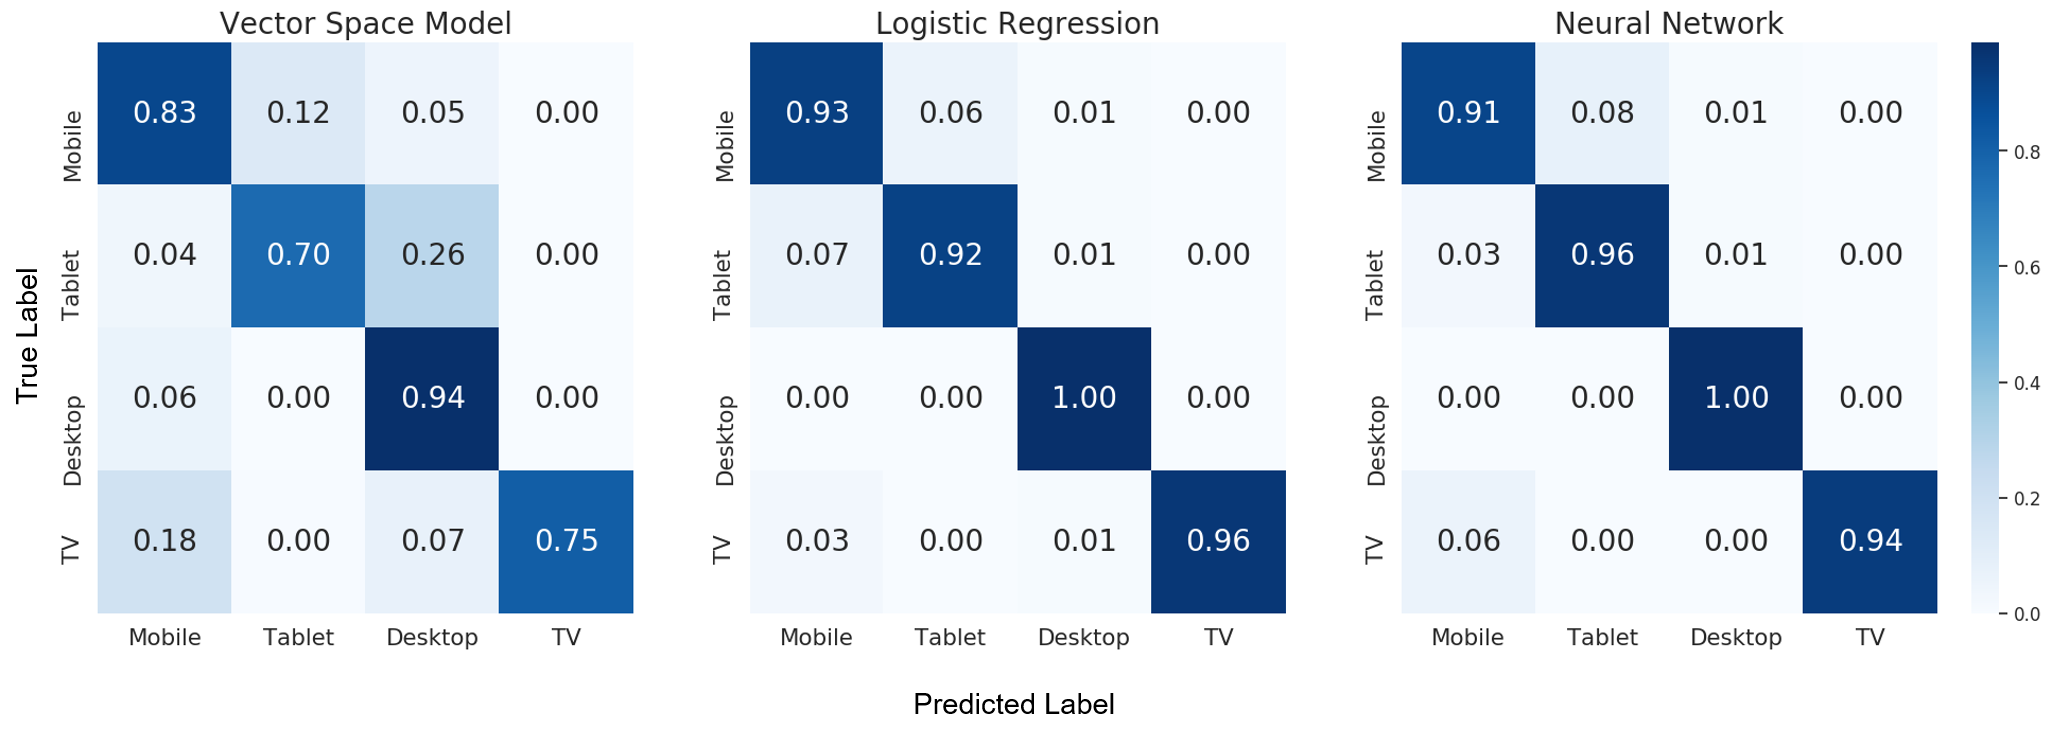
\includegraphics[width=1\textwidth]{Conf_text.png}
	\caption{Accuracy by device and method}\label{fig:devAcc}
\end{figure}

The performance was tested by checking the time required by each method:
\begin{itemize}
	\item To provide the result of a prediction: Table \ref{tab:querytimes} provides the average value for each method. As can be seen, vector space model method was much slower than the other ones returning a result, since it had to calculate the similarity of the query with all the User Agents in the dataset. Logistic regression and neural network present similar results. In these cases, the computational cost of the classification was much lower than in the former. All in all, the three methods could be valid when talking about response time, since the obtained values would not affect the user experience. 
	\item To train the employed model: Table \ref{tab:traintimes} provides the average value for each method. As expected, the vector space model was the method that requires the least time. The reason was that it does not strictly learn, but it tokenises the dataset and calculates the weight of each term of the User Agents in order to have a prepared dataset when a query is received. Logistic regression was the second fastest model. Its learning process consists on updating the coefficients of a polynomial expression according to the terms of the User Agents in the dataset. It needed seven times the time needed by the vector space model, but the obtained accuracy was considerably better. Finally, neural network method was the slowest training the model and it needed approximately seven times the time needed by the logistic regression to train the model. However, as training is a one-time cost, this result does not exclude neural networks as being a candidate method for device type detection. More complex User Agent strings will increase the overhead, but it is not easy to envisage a real scalability problem.
\end{itemize}

\begin{table}
	\centering
	\caption{Average time required to process the result of a prediction (on CPU)}
	\label{tab:querytimes}
	\begin{tabular}{||c|c|c||}
		\hline
		\textbf{Method} & \textbf{Time average (s)} & \textbf{$\sigma^2$}\\
		\hline
		Vector space model & 0.0512 & 1.1818E-07\\
		Logistic regression & 0.0006 & 1.19E-07\\
		Neural network & 0.0007 & 2.52E-08\\    
		\hline
	\end{tabular}
\end{table}

\begin{table}
	\centering
	\caption{Average time required to process or learn on the initial dataset (on CPU)}
	\label{tab:traintimes}
	\begin{tabular}{||c|c|c||}
		\hline
		\textbf{Method} & \textbf{Average time (s)} & \textbf{$\sigma^2$} \\
		\hline
		Vector space model & 4.1186 & 0.1683\\
		Logistic regression & 29.91243 & 0.3169\\
		Neural network & 212.2969 & 2.1452 \\    
		\hline
	\end{tabular}
\end{table}



Additionally, the potential of improvement was analysed. There are several possibilities to improve the accuracy results obtained by the methods described, probably being the neural network approach method that can be improved the most since enhancements can be applied across several dimensions. For instance, tuning the hyperparameters of the network (number of layers, dropout rate, etc.) is a standard way of increasing the network performance. Recurrent neural network architectures such as LSTM \cite{gers1999learning} are more suited for processing of text sequences as they keep memory of previous input data and thus are likely better than a standard neural network as the one presented above.

Therefore, in this part of the research we used the information about the device made available by the browser to implement device typification. 
Nevertheless, there are device properties that are related to usage patterns, such as the degree of privacy of a device, which cannot be obtained from the browser and have not been integrated in our implementation.
For this prototype implementation, we will use three of the device properties defined in Section~\ref{devices}: screen size, input capabilities and processing capabilities.
Since the screen size is a key property for layout generation, we will provide a specific definition for this property in Section~\ref{Imp-s2}.

\subsection{Layout templates and properties} \label{imp_lay}

In Section~\ref{layouts} we described a strategy to reduce the combinatorial possibilities in the generation of layouts. 
Following the usual typification approach, a reduced set of template layouts is used. 

The template to be used in each specific situation will depend on a huge range of parameters and criteria that have to be analysed, such as the device type, the number of components to be shown, the empty space in the screen or the possibility of overlapping components. 

\subsubsection{Analysis of parameters in layout templates} 
In order to guide the research and analyse the parameters to take into account when choosing a layout template, a study was carried out and published in \cite{zorrilla15bmsb}. The following subsections summarise the cited work focusing on the user tests conducted and the results obtained.  

\paragraph{User tests}

The main objective of the user tests was to see the effect of the following parameters in the user interface:
\begin{itemize}
	\item \textbf{The device}: As happens in a single-device application, the target device is very relevant to build a responsive Web application. In the same way, the devices involved in a multi-device application are expected also to be relevant. 
	\item \textbf{The number of Web Components}: The quantity of pieces of information to be shown in that device can affect on how to present the content.
	\item \textbf{The nature of the application}: This parameter could be important to decide the arrangement of the user interface. For instance, if there is a main video and related information on the device, or if the video is being displayed on another device and that device is being used only for extra information.
	\item \textbf{Other devices being used at the same time}: We wanted to know if having a second device being used simultaneously has an impact on how the user wants to arrange the components in the first screen. 
\end{itemize}


To find out the influence of each parameter, they were enclosed to these options: 
\begin{itemize}
	\item \textbf{The device}: Three different devices. A Motorola Moto G Smartphone in portrait mode, A Nexus 10 tablet in landscape mode, and a Samsung UE40C8000 TV.
	\item \textbf{The number of components}: Showing three or six components at the same time.
	\item \textbf{The nature of the application}: Two different scenarios. At least one of the components was a video, or there was not a video among the components.
	\item \textbf{Other devices being used at the same time}: Two possible situations. The evaluated device was the only one being used by the user or there was another device as a companion screen.
\end{itemize}
Testing images have been created simulating a broadcasted live F1 race scenario with all the possible combinations of the first three parameters (see Table \ref{tab:table1bmsb15} from Id 1 to 12).

\begin{table}[h!]
	\centering
	\caption {Combinations with the defined parameters} \label{tab:table1bmsb15} 
	\begin{tabular}{ ||M{2cm}|M{2.5 cm}|M{2 cm}|M{3 cm}|M{2 cm}|| }
		\hline		 
		\bf Id & \bf The device & \bf The number of components & \bf The nature of the application & \bf Other devices being used at the same time\\
		\hline
		1 &	TV & 3 &	At least one video &	No\\
		2 &	TV & 6 &	At least one video	& No\\
		3 &	TV & 3 & No videos &	No\\
		4 &	TV & 6 &	No videos &	No \\
		5 &	Tablet & 3 & At least one video & No \\
		6 &	Tablet & 6 & At least one video & No \\
		7 &	Tablet & 3 & No videos &	No \\
		8 &	Tablet & 6 & No videos &	No \\
		9 &	Smartphone & 3 & At least one video & No \\
		10 & Smartphone	& 6	& At least one video & No \\
		11 & Smartphone	& 3	& No videos &	No \\
		12 & Smartphone	& 6	& No videos &	No \\
		13 & Tablet & 3	& At least one video &	Yes, A TV \\
		14 & Tablet	& 6	& At least one video &	Yes, A TV \\
		15 & Tablet	& 3	& No videos &	Yes, A TV \\
		16 & Tablet	& 6	& No videos	& Yes, A TV \\
		
		\hline
	\end{tabular}
\end{table} 

Apart from these 12 context situations, four more were created to evaluate the “Other devices being used at the same time” parameter. A TV showing two fixed components was used and different contexts were presented in a tablet, making the user think about how to present the content in the tablet, while they were also watching related content in the TV. These situations are also represented in Table \ref{tab:table1bmsb15} from Id 13 to 16.

For each one of the 16 combinatorial contexts, always four different user interface arrangement patterns were created:
\begin{itemize}
	\item \textbf{Grid Layout}: Based on the CSS Grid Layout Module Level 1\footnote{\url{http://dev.w3.org/csswg/css-grid/}}  (see example in Figure \ref{fig:layexampBMSB15}a).
	\item \textbf{Picture-in-picture Layout (PiP)} (see example in Figure \ref{fig:layexampBMSB15}b).
	\item \textbf{Menu Layout} (see example in Figure \ref{fig:layexampBMSB15}c).
	\item \textbf{Horizontal Layout} (see example in Figure \ref{fig:layexampBMSB15}d).
\end{itemize}
\begin{figure}
	\centering
	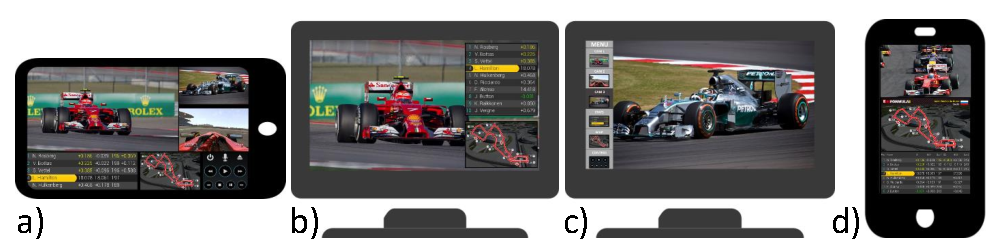
\includegraphics[width=1\textwidth]{layoutsexamples.pdf}
	\caption[Layouts examples]{a) A grid template layout example on a tablet in the context with ID number 6. b) A PiP template layout example on a TV in the context with ID number 1. c) A menu template layout example on a TV in the context with ID number 2. d) A horizontal template layout example on a smartphone in the context with ID number 9.}
	\label{fig:layexampBMSB15}
\end{figure}

The tests were done with 47 users, one by one, being always an expert presenting each one of the 16 context situations. The expert gave them a very brief description of the context and four images showing the components organised according to each layout. Then he asked the participants for each context:

\begin{center}
\textit{Which layout would you choose on this moment to see the F1 race?}
\end{center}

All the tests were carried out in the Digital Home Lab of Vicomtech, where there is a similar environment on what it can be find on a living room. From the 47 users, 40 of them were researchers, with expertise on different fields, and 7 of them were administrative staff people. It took around 15 minutes to perform the test with each user, so around 12 hours in total, divided in three different days. Figure \ref{fig:usertestsBMSB15} presents pictures took during the tests.
\begin{figure}
	\centering
	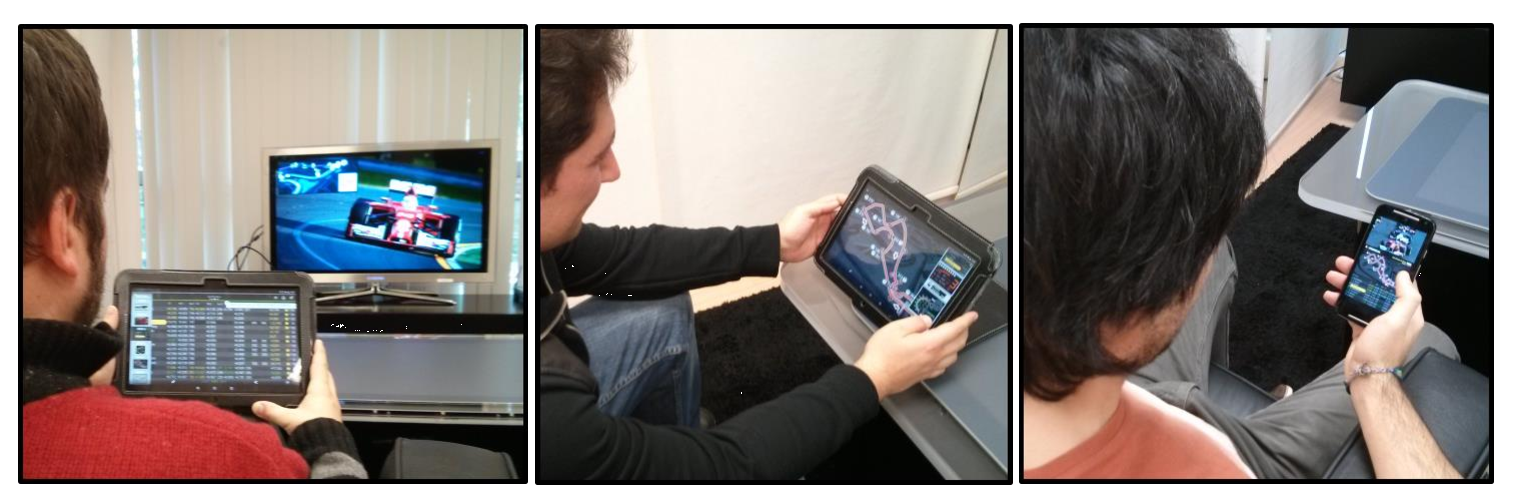
\includegraphics[width=1\textwidth]{usertests.pdf}
	\caption[User tests images]{Images from user tests. In the left a user in front of the context situation with ID number 16 with the menu layout on the tablet. In the middle a user with the context situation with ID number 16 with the PiP layout in the tablet and in the right a user in the context situation with ID number 9 with the horizontal layout on the smartphone.}
	\label{fig:usertestsBMSB15}
\end{figure}
\paragraph{Results of the user tests and conclusions}
Table \ref{tab:table2bmsb15} presents the answer that the users gave for each one of the 16 contexts. 
\begin{table}[h!]
	\centering
	\caption {Results of the chosen layouts on each situation} \label{tab:table2bmsb15}
	\begin{tabular}{ ||K{2 cm}|K{2 cm}|K{2 cm}|K{2 cm}|K{2 cm}|| }
		\hline	
		\bf \multirow{3}{*}{Context Id}  & \multicolumn{4}{c||}{\bf Results} \\
		& \multicolumn{4}{c||}{\bf Number | Percentage of users choosing each layout}\\
		\cline{2-5}
		& \bf Grid & \bf Pip & \bf Menu & \bf Horizontal\\
		\hline
		1 &	19 | 40\% &	13 | 28\% &	14 | 30\% &	01 | 02\% \\
		2 &	32 | 68\% &	08 | 17\% &	06 | 13\% &	01 | 02\% \\
		3 &	28 | 60\% & 16 | 16\% &	03 | 03\% &	00 | 00\% \\
		4 &	33 | 70\% &	07 | 15\% &	05 | 11\% &	02 | 04\% \\
		5 &	09 | 19\% &	26 | 55\% &	11 | 23\% &	00 | 00\% \\
		6 &	34 | 72\% &	08 | 17\% &	05 | 11\% &	00 | 00\% \\
		7 &	23 | 49\% &	14 | 30\% &	07 | 15\% &	03 | 06\% \\
		8 &	31 | 66\% &	09 | 19\% &	07 | 15\% &	00 | 00\% \\
		9 &	05 | 11\% &	04 | 09\% &	20 | 43\% &	18 | 38\% \\
		10 & 22 | 47\% & 03 | 06\% & 19 | 40\% & 03 | 06\% \\
		11 & 11 | 23\% & 08 | 17\% & 09 | 19\% & 19 | 40\% \\
		12 & 16 | 34\% & 08 | 17\% & 15 | 32\% & 08 | 17\% \\
		13 & 17 | 36\% & 17 | 36\% & 13 | 28\% & 00 | 00\% \\
		14 & 28 | 60\% & 07 | 15\% & 10 | 21\% & 02 | 04\% \\
		15 & 30 | 64\% & 06 | 13\% & 10 | 21\% & 01 | 02\% \\
		16 & 33 | 70\% & 03 | 06\% & 11 | 23\% & 00 | 00\% \\	
		
		\hline
	\end{tabular}
	
\end{table} 
Moreover, it was analysed the behaviour of each one of the users when one of the parameters changed, in order to evaluate which parameter changed their mind. This measured if the user selected a different layout when the context changed. Analysing the relevance of each one of the four parameters defined, we concluded that all of them are important and have a big impact above 45\%. This means that at least 21 of the 47 users tested change the mind when one of the parameters changes in the context.

Figure \ref{fig:impactparamBMSB15} shows that the most relevant parameter is the device, with an impact above 59\%. As happens for “single device” application, it was also expected to be an important parameter for multi-device applications, where the user is consuming an application from more than one device at the same time. The number of components is also very relevant being around 5 percentage points below. This means that it is important to change the arrangement of the user interface depending the outcome of the adaptation engine while the number of components to be shown changes.

\begin{figure}
	\centering
	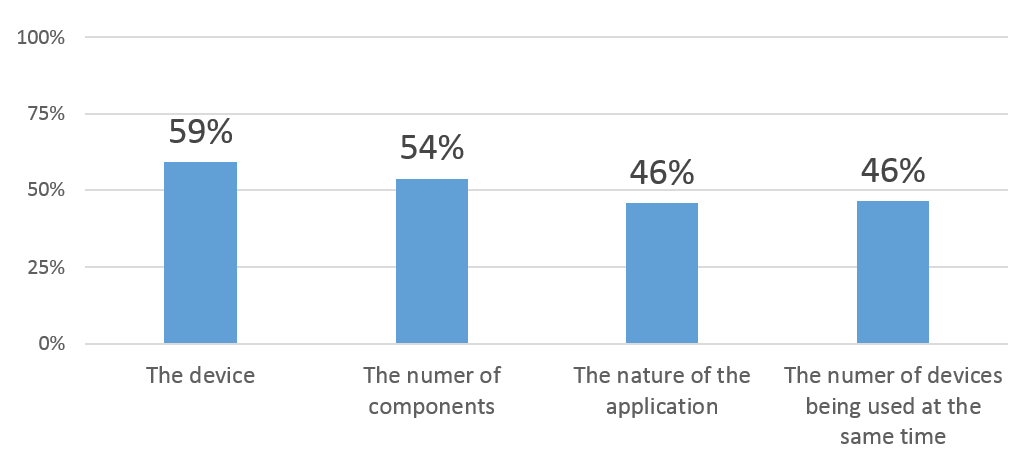
\includegraphics[width=1\textwidth]{impactparam.pdf}
	\caption[Relevance of the four defined parameters]{Relevance of the four defined parameters}
	\label{fig:impactparamBMSB15}
\end{figure}
The nature of the application and the number of devices being used at the same time are also relevant parameters, both of them around 46\%, to take them into account to develop the final software of the UI Engine.

These results have been published in \cite{zorrilla15bmsb} and provide a valuable information in order to have a notion of how a layout should be chosen when creating responsive user interfaces for Web-based multi-device media services. However, the results are not conclusive. In order to obtain more accurate results, further research and more formal user tests are needed, using a real multi-device service instead of images simulating it, widening the range of layouts analysed and performing the tests with a higher sample of users with different profiles. Even so, the tests were useful to lay the foundation of the research. They showed that while PiP and menu layouts are more neutral, grid layout is very dependent of the components that constitute it. In this context, a deeper analysis of the grid layout revealed that there are some parameters that make a layout more or less attractive, such as the scrolling, the empty space or the overlaps. Therefore, instead of a concrete layout it is important to see that there are some criteria behind each layout that are related to the parameters in Figure \ref{fig:impactparamBMSB15}. For that reason, for the prototype implementation, we choose a set of layout templates of standard use in current applications and devices, each one being representative for a criteria. 
These are Picture-in-Picture (Figure \ref{fig:layouts}A), Split (Figure \ref{fig:layouts}B) and Carousel (Figure \ref{fig:layouts}C), which we describe in terms of the properties we defined in Section~\ref{layouts}:

\begin{enumerate}
	\item \textbf{Picture-in-Picture (PiP)}: space sharing template in which a component is shown in full screen and the others are overlapped with a smaller size over the first one. PiP shows all the components at the same time to the detriment of the shown area of the first component (overlapped) and the resolution of the secondary components. 
	\item \textbf{Split}: space sharing template in which the screen is divided into a regular grid according to the number of components. Unlike PiP, there is no overlapping. However, empty space appears when the number of components does not match the number of cells established by the template.
	\item \textbf{Carousel}: time sharing template in which all the components are organised in a carousel that allows to left- or right-slide all the elements. Carousel is commonly used for image galleries. 
\end{enumerate}

\begin{figure}	
	\begin{center}
		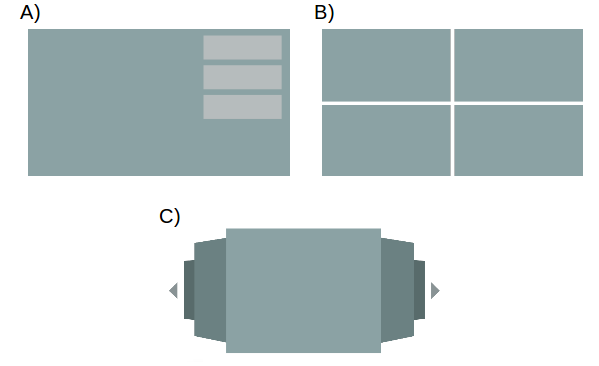
\includegraphics[width=0.48\textwidth]{layouts.png}
		\caption{Considered layout templates}
		\label{fig:layouts}
	\end{center}
\end{figure} 

A summary of the template layout properties is shown in Table~\ref{tab:layoutprop}. These properties derive from the experience achieved in the previous study. 



\begin{table}
	\centering
	\caption {Layout properties for each template}\label{tab:layoutprop}
	\begin{tabular}{||l|c|c|c||}
		\hline
		\textbf{Property} & \textbf{PiP} & \textbf{Split} & \textbf{Carousel} \\
		
		\hline
		\textbf{Time sharing} & \xmark & \xmark & \cmark \\
		\hline
		\textbf{Space sharing} & \cmark & \cmark & \xmark \\
		\hline
		\textbf{Overlapping} & \cmark & \xmark & \xmark \\
		\hline
		\textbf{Scrolling} & \xmark & \xmark & \xmark \\
		\hline 
		\textbf{Distortion} & \cmark & \cmark & \cmark \\
		\hline
		\textbf{Prior components} & \cmark & \xmark & \xmark \\
		\hline 
	\end{tabular}
\end{table}


Observe that, contrary to components and devices, for layouts the typification function $\mathcal{T^L}$ does not have practical interest. 
Instead, in an implementation the aim is, given a template $t$, finding a layout $l$ such that $\mathcal{T^L}(l)=t$ and that $l$ ranks a high quality in terms of the layout quality criteria explained in Section~\ref{s2}. Therefore, ideally $l=l^*$. 


\subsection{Implementing assignation} \label{imps1}
Step~1 of the adaptation process uses the vectors of properties for both components and devices to calculate affinities on the basis of the affinity matrix defined in~\ref{s1}.

In a real deployment, the matrix values should be carefully set, which involves extensive user evaluation and/or a continuous adaptive learning process.
However, the scope of the present work is aimed at the formulation and validation of an adaptation model. Hence, we have built the affinity matrix with values obtained by polling a reduced community of users. 

Once the affinity matrix and property vectors have been set, the implementation of Step~1 is quite straightforward. 
Flexible data structures have been implemented to allow for adding or removing components or devices and evaluating all their properties. 

To assign a given component, once the affinity vectors for each target device were obtained as represented in Figure~\ref{fig:reqgraph}, we follow these criteria:
\begin{enumerate}
	\item Choosing a device fitting every property, or the highest amount of them. In our example, the TV would be the selected device for the main programme component (see Figure \ref{fig:chartcase1}).
	\item  Minimising under-fitting values. In our example, in absence of a TV, we would assign the component to the smartphone.
	\item Finally, over-fitting values are considered, choosing the device whose affinity values are the closest to the requirement values.
\end{enumerate}

\begin{figure}
	\begin{center}
		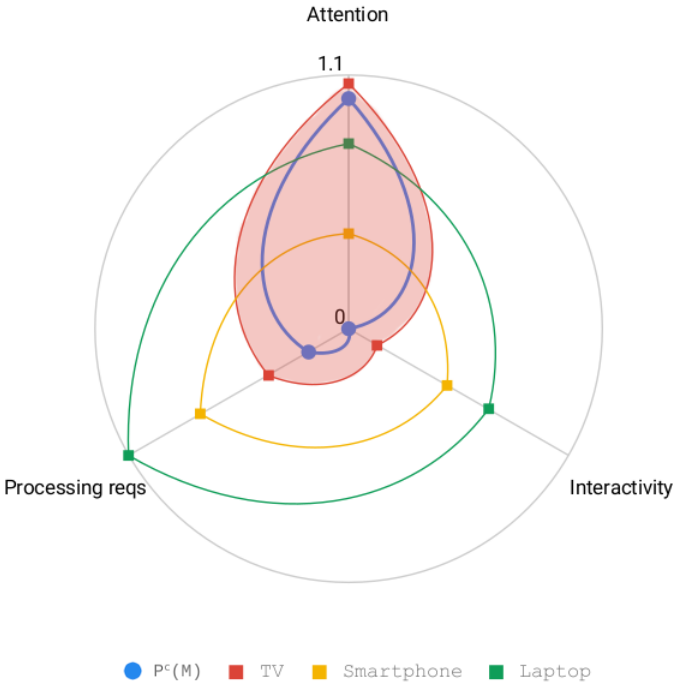
\includegraphics[width=0.55\textwidth]{chartcase1.png}
		\caption{The device fitting every property}
		\label{fig:chartcase1}
	\end{center}
\end{figure}

\begin{figure}
	\begin{center}
		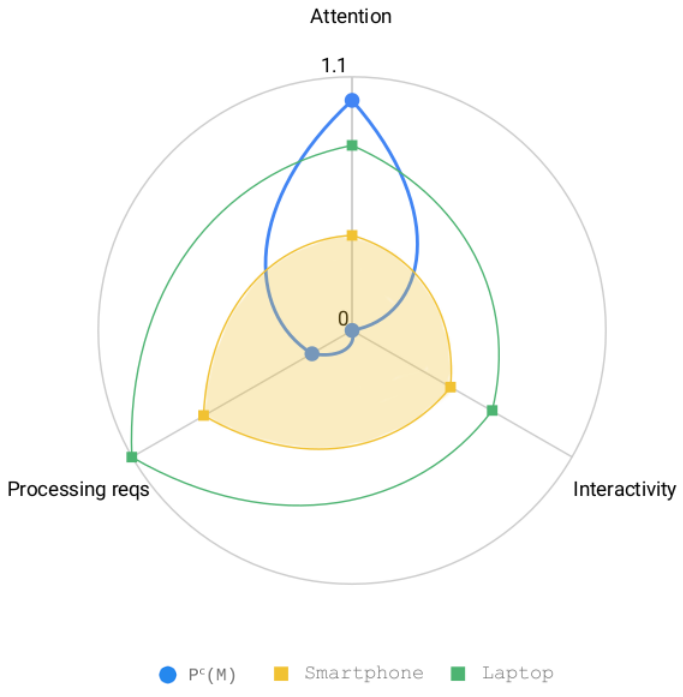
\includegraphics[width=0.55\textwidth]{chartwithoutTV2.png}
		\caption{Maximising the usage of resources when there is no TV}
		\label{fig:chartwithoutTV}
	\end{center}
\end{figure}

Different implementations could choose different criteria. An alternative implementation could consider only the scalar affinity value following Eq. \ref{Eq:affinity}. In this case the affinity values would be $\mathcal{A}(M,tv) = 1.14$, $\mathcal{A}(M,smartphone) = 0.558$ and $\mathcal{A}(M,laptop) = 1.02$, being the TV the best device, followed by the laptop and being the smartphone the last one. Another implementation could be interested in maximising the usage of resources. Following with the same example, with this implementation the TV would be the best device, while in its absence the component would be assigned to the smartphone and the laptop would be discarded as it would lead to wasting processing and interactivity resources (see Figure \ref{fig:chartwithoutTV}).


\subsection{Implementing representation}
\label{Imp-s2}

Step~2 uses the assignments obtained in Step 1 to calculate the layout template in each device. 
%For the sake of the simplicity, 

Our prototype implementation for layout selection is based on the screen size property of the device types (we will add the property of input capabilities in Section~\ref{val}).
To properly define the screen size property, we considered the \emph{screen apparent area}, denoted as $S$. 

To measure the apparent area of a screen with diagonal $h$ meters and a normalised 1:1 aspect ratio, we situate the screen at the usual watching distance and calculate the projected area of the screen to distance 1 meter.
Note that this results in more realistic relations than the ones obtained comparing raw screen areas.
For example, a screen with a diagonal size $h$ situated at a distance of $l$ meters from the user has the same apparent area as a $kh$ screen at $kl$ meters.
%First of all, to parameterise how the layout templates can be deployed across the different device types, an analysis of the apparent area of each device has been done, which takes into account basically the screen size, and the user distance and 

Resolution has been ignored for the screen size definition, since it is not a constraint in current devices. 
However, some ergonomic aspects should be considered in real deployments. 
For example, for similar apparent sizes, a TV would provide a more comfortable viewing distance for the user's eyes, while smartphones or tablets can be brought nearer more easily. 


Table~\ref{tab:aparea} shows an example of the estimated apparent areas for the four considered device types as well as some related parameters that we explain next. 

A relevant parameter for layout generation, specifically for the Split template, is the minimum apparent size of a component to be comfortably seen by the user, denoted as $S_c$.
Indeed, this is a user-related parameter that would deserve extensive user evaluation, in addition to the ability for configuration and adaptation from user context parameters. 
To provide an example to illustrate the prototype implementation of our adaptation model, we will set $S_c$ to 0.02 square meters.
This results, for example, in one half of a smartphone screen at 40cm from the user.
For the other devices, Table~\ref{tab:aparea}
shows the number of minimum size components that would fit into the screen, i.e., $S/S_c$, conveniently rounded to an integer number.
\newcolumntype{M}[1]{>{\centering\arraybackslash}m{#1}}

\begin{table}
	\centering
	\caption {Parameters related to apparent areas of screens}\label{tab:aparea}
	\setlength{\extrarowheight}{0.05cm}
	\begin{tabular}{||M{5cm}|M{2.5cm}|M{2cm}|M{2cm}|M{1cm}||}
		\hline
		\textbf{Device} & \textbf{Smartphone} & \textbf{Tablet} & \textbf{Laptop} & \textbf{TV}\\
		
		\hline
		\textbf{Screen diagonal (cm)} & 12.5 & 25 & 35 & 150\\
		\hline
		\textbf{User distance (cm)} & 40 & 50 & 60 & 250\\
		\hline
		\textbf{Angle (degrees)} & 17.36 & 26.58 & 30.25 & 30.93\\
		\hline
		\textbf{Apparent area, $S$ ($m^2$)} & 0.044 & 0.100 & 0.127 & 0.132\\
		\hline
		\textbf{Comp. min size, $S_c$ ($m^2$)} & 0.02 & 0.02 & 0.02 & 0.02\\
		\hline
		\textbf{N. of components, $\floor*{S/S_c}$} & 2 & 4 & 6 & 6 \\
		\hline
	\end{tabular}
\end{table}

For PiP layouts, two additional parameters are required: the fraction of the screen area devoted to inserting the overlapped secondary components, $F_i$, and the size of the secondary components, $S_s$ which in general can be smaller than $S_c$.
Note that $F_iS/S_s$ denotes the maximum number of insertions in a PiP layout. 
Table~\ref{tab:layoutparam} summarises the values for the three templates adopted in the implementation of Step~2.

\begin{table}
	\centering
	\caption {Screen related layout parameters}\label{tab:layoutparam}
	\begin{tabular}{||l|c|c|c||}
		\hline
		\textbf{Parameter} & \textbf{PiP} & \textbf{Split}  & \textbf{Carousel}\\
		
		\hline
		\textbf{Max N. of main comp.}  & 1 & $S/S_c$ & 1\\
		\hline  \textbf{Insertion frac., $F_i$}  & 0.33 & 0 & 0 \\
		\hline
		\textbf{Insertion min size, $S_s$}  & $S_c/3$ & NA & NA\\
		\hline
		\textbf{Max. N. of insertions}  & $F_i S/S_s$ & 0 & 0 \\
		\hline
		% \textbf{T} & 1 & 0 & 0 \\
		% \hline
	\end{tabular}
\end{table}

We have implemented three criteria for the evaluation of the layout quality, according to the evaluation model introduced in Section~\ref{layouts}:

\begin{itemize}
	\item \textbf{Rate of the components shown ($\alpha_1$)}: This criterion evaluates the portion of the components that is shown in the display, and refers to three different aspects: (a) the portion of the number of components, (b) the portion of the component area, and (c) the portion of time that a component is shown.
	Note that Split layouts rank the highest in every aspects, while PiP is penalised in (b) by the overlapped area of the main component, and the time sharing layouts, such as Carousel, are penalised in (c) for the time slice where components are shown.
	\item \textbf{Representation of every shown component in its entirety ($\alpha_2$)}: This criterion is related with how the components shrink to fit to a specific space slot in the space-sharing layouts. The criterion ranks the maximum for Carousel, while it can penalise Split and PiP in two different aspects: (a) shrink in the scale of a component, and (b) distortion of the aspect ratio of the component (the last aspect has not been considered in our example implementation).
	\item \textbf{Efficiency in the use of the screen area ($\alpha_3$)}: Although we are allowing some degree of distortion, in Split layouts the screen is divided in a regular grid that, for practical reasons, excludes extreme configurations (e.g., many components in a single row). As a consequence, for some specific numbers of components, an unused screen area will be generated, which is accounted for as lost space and penalises this criterion.  
\end{itemize}

Observe that the above criteria, in the framework of the adaptation model defined in Section~\ref{ad}, allow not only for the evaluation of the three pure layout templates we are considering for the implementation but also for a combinatorial of hybrid layouts, as, for instance, a carousel showing several components simultaneously, as well as many others. 

Once the three criteria have been defined, the quality of each layout can be calculated as shown in Eq. \ref{Eq:layoutq}. 
We have performed an empirical set up of the internal coefficients in the equation to obtain intuitively realistic outcomes, resulting in the quality graphs in Figs.~\ref{fig:laygraphS}, \ref{fig:laygraphT} and \ref{fig:laygraphLTV} for each device type in terms of the number of components to show.
The coefficient used for each of the aforementioned criteria has been $w_1=1.4$, $w_2=0.3$ and $w_3=1.2$ respectively.

Observe that time-sharing layouts (Carousel) maintain a significant quality level for a high number of components whereas space-sharing layouts (PiP and Split) are more suitable for a low number of components,
depending on the particular election on the device type and the efficient fit of the components in the screen (e.g. the quality decreases sharply for Split layout when the number of components cannot be arranged in a grid occupying the entire screen).

In a real deployment, the user can be given a way to control the relative relevance of each criteria.
Furthermore, an exhaustive user evaluation or an adaptive learning process could find the most appropriated values for the specific deployment and user profile, showing at the same time the power of generalisation of our model. 
Regarding the last point, in Section~\ref{val} we will show the ability of the model to easily accept extensions and modifications, specifically for including new criteria or properties. 

\begin{figure}
	\begin{center}
		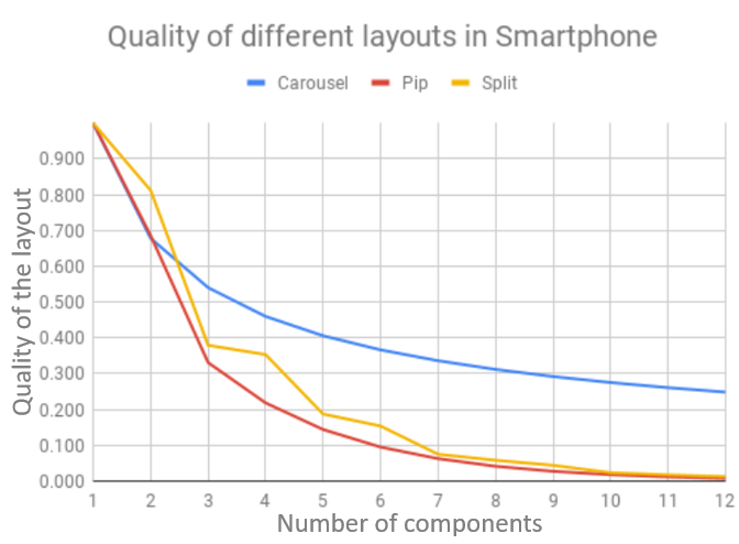
\includegraphics[width=0.65\textwidth]{QSP.png}
		\caption{Quality of the layouts in Smartphone in terms of number of components}
		\label{fig:laygraphS}
	\end{center}
\end{figure}

\begin{figure}
	\begin{center}
		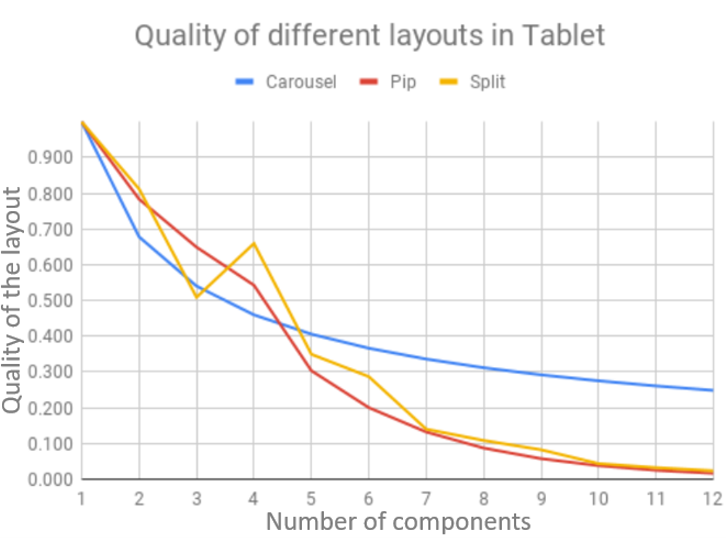
\includegraphics[width=0.65\textwidth]{QT.png}
		\caption{Quality of the layouts in Tablet in terms of number of components}
		\label{fig:laygraphT}
	\end{center}
\end{figure}

\begin{figure}
	\begin{center}
		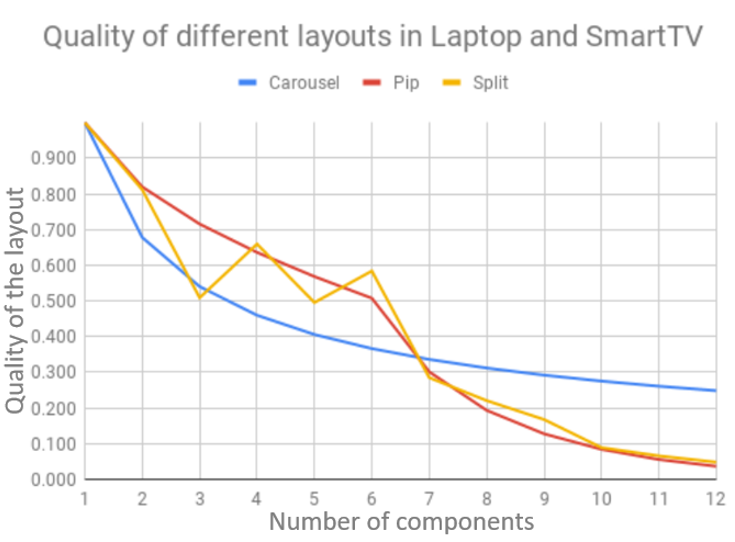
\includegraphics[width=0.65\textwidth]{QTV.png}
		\caption{Quality of the layouts in Laptop and Smart TV in terms of number of components}
		\label{fig:laygraphLTV}
	\end{center}
\end{figure}

\subsection{The role of context: triggering the adaptation process}\label{ctx}

\label{Triggering}
In the previous subsections we have described an implementation of the two-step process. 
The question now is when the adaptation process should be launched, either from the beginning or only from Step 2 in some specific devices. 
To address this issue we use context information. 

The information about contextual factors and external event occurrences while using a service is usually referred to as context \cite{hussain2018model}. 
In our system, context changes are used to trigger the adaptation process in such a way that the system can update and maintain the user experience at convenient levels. 

Usually, context is divided in three parts: user context, physical context and system context. 
In our scenario, the user context includes user preferences and user state (e.g., mood or stress level). 
We will also consider explicit interaction as the user context updates. 
Physical context parameters can include the location, time, ambient light, and noise level. 
Finally, the system context is determined by the state parameters of the devices, including the battery level, connectivity conditions, etc. 

As usual, context information is mainly based on sensors and can be elaborated and interpreted by a learning process. 
In this way, a complete context service could be built on top of our system to boost sophisticated smart environments. 
Nevertheless, for the scope of this work, we manage context information as an asynchronous sequence of events.
Either directly or indirectly, an event of the sequence is able to promote a run of the adaptation process.

To complete the picture (refer to Fig.~\ref{fig:overview}), our multi-device adaptation environment can be implemented as an event-driven system where events can be produced by different Situations:

\begin{enumerate}
	\item A change in the component set $C$. This change can be produced by the broadcast programme or by an action of the user moving a component from one device to another. As an incremental modification, only Step~2 will be executed in the involved devices.
	\item Joining or leaving a device in the device set $D$, generally involving a rerun of the adaptation process. 
	\item A context update. For example, when a viewer moves away from the TV, the adaptation process could begin the smartphone to move from a complementary screen to the main element in $D$. To mention another example, the adaptation process could be triggered in the case of a low battery level in a device, forcing a Situation-2 event.
	\item In some cases, described next, an internal event can trigger a complete rerun of the adaptation process. 
\end{enumerate}

The last of the situations refers to the fact that the two-step incremental adaptation process could sometimes lead to an unbalanced assignation of components on devices.
Devices with many components assigned could rank low for every layout templates in Step~2 and, furthermore, overloaded devices could suffer resource exhaustion, resulting in poor performance, such as in video rendering. 

A strategy to avoid this situation is considering resource availability in each device as a system context parameter. 
When a resource is almost exhausted, an internal event is produced to rerun the entire adaptation process. 
Note that the strategy should be complemented with the introduction of the resource availability context parameter as a criterion in the assignation step. 
As Step~1 is implemented iteratively, a low value for resource availability in a device will prevent assigning a new component to the device despite the affinity value.



\section{Validation}\label{val}

This section provides a validation of the proposed methodology for the user interface adaptation of multi-device media services regarding three different aspects: quality, efficiency and universality. On one hand, the quality and the efficiency are validated through the evaluation of the two-step adaptation process with experiments that compare the sub-optimal outcome with the optimal adaptation solution (which requires exploring the whole solution tree), analysing the trade-off between the adaptation quality and the computation effort for a responsive implementation. 
On the other hand, the universality of the proposed methodology is evaluated taking as a reference an environment based on the real deployment described in Chapter \ref{chap:deployment} and analysing its limitations towards the versatility and flexibility to fit to novel properties, components, devices, use cases, etc. As described in Chapter \ref{chap:introduction}, the lessons learned with the pilot programme have been the starting point to develop the hypotheses of this work. In the same way, it has been useful to synthesise the use cases addressed in this section which are seen as a tool to validate the developed adaptation model.

Figure \ref{fig:deployment_example} shows a picture of a scenario extracted from the deployment where a viewer consumes a multi-device TV programme delivered by a broadcaster. A set of use cases derived from this scenario will be used in the following subsections.

\begin{figure}
	\begin{center}
		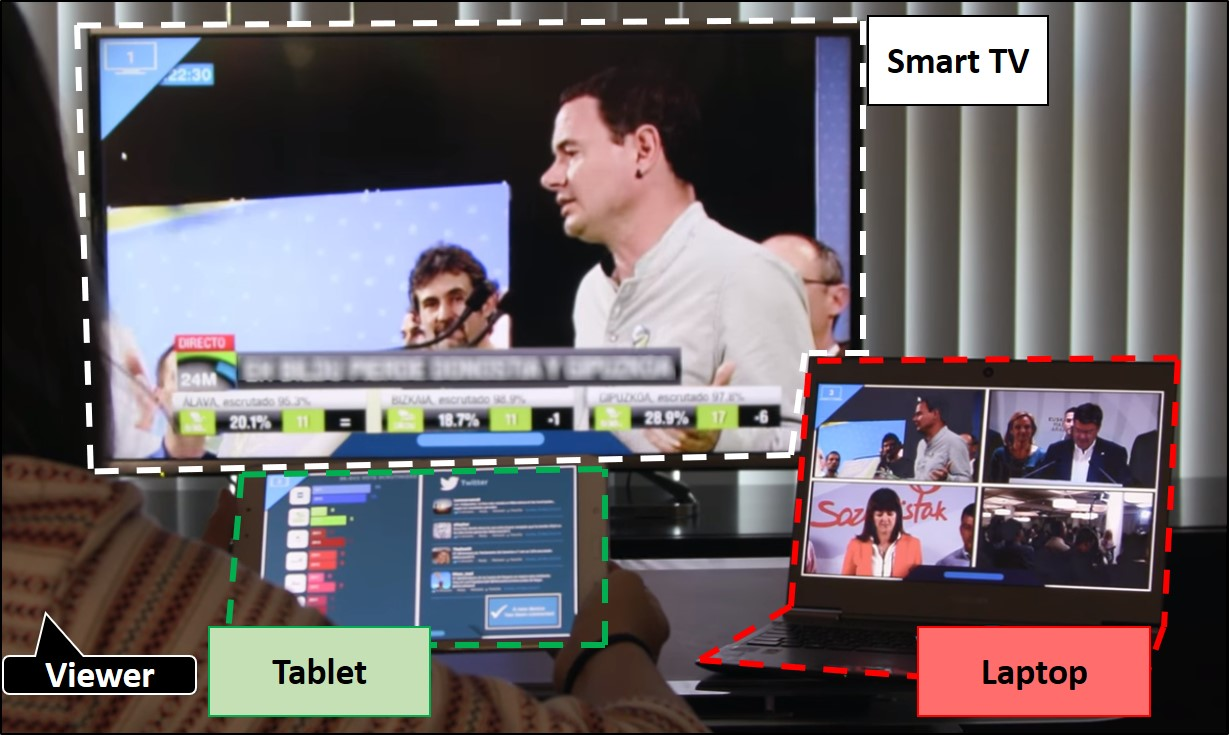
\includegraphics[width=1\textwidth]{Deployment.jpg}
		\caption{A picture of the deployment of a multi-device media service}
		\label{fig:deployment_example}
	\end{center}
\end{figure} 

\subsection{Evaluating the quality of the adaptation process}

To evaluate the two-step adaptation process, the proposed model has been implemented \cite{modelGit} defining a set of components, a set of available devices, a set of available layout templates, and defining representative properties and parameters for all the user interface elements. 

On the one hand, five properties have been defined and evaluated for each of the components. Table \ref{tab:compprop} shows the parametrisation performed in the implementation for all the component types identified in \cite{dominguez2018componentizing}.


\begin{table}
	\centering
	\caption {Summary of used component types and properties}\label{tab:compprop}
	\begin{tabular}{||M{1.8cm}|M{1.6cm}|M{2.2cm}|M{1.9cm}|M{1.9cm}|M{2.6cm}||}
		\hline
		\textbf{Properties} & \textbf{Attention} & \textbf{Interactivity} & \textbf{Processing req} & \textbf{Broadcast req} & 
		\textbf{Confidentiality} \\
		
		\hline
		\textbf{Main} & 1 & 0 & 0.3 & 1 & 0 \\
		\hline
		\textbf{Sec. videos} & 0.7 & 0.3 & 0.9 & 0 & 
		0.1 \\
		\hline
		\textbf{Banner}& 0.8 & 0.2 & 0.1 & 0 & 
		0.1 \\
		\hline
		\textbf{St Data} & 0.6 & 0.2 & 0.2 & 0 & 
		0.3 \\
		\hline 
		\textbf{Dyn Data} & 0.6 & 1 & 0.3 & 0 & 
		0.8 \\
		\hline
		\textbf{Social} & 0.3 & 1 & 0.3 & 0 & 
		1 \\
		\hline
		\textbf{UGC} & 0.3 & 1 & 0.7 & 0 & 
		0.9 \\
		\hline
		
		\textbf{Adv} & 0.9 & 0 & 0.5 & 0.8 & 
		0  \\
		\hline
		
	\end{tabular}
\end{table}


On the other hand, four available connected devices have been parameterised and, again, five different properties have been defined for each device type. Table \ref{tab:devprop} shows the parametrisation performed in the implementation for all the identified device types. 

\begin{table}
	\centering
	\caption {Summary of used device types and properties} \label{tab:devprop}
	\begin{tabular}{||c|c|c|M{1.9cm}|c|M{1.9cm}||}
		
		\hline
		\textbf{Properties} & \textbf{Screen size} & \textbf{Input cap.} & \textbf{Processing cap.} & \textbf{Privacy} & \textbf{Broadcast cap.} \\
		\hline
		\textbf{Smartphone} & 0.2 & 0.7 & 0.6 & 1 & 0\\
		\hline
		\textbf{Tablet} & 0.6 & 0.8 & 0.7 & 1 & 0\\
		\hline
		\textbf{Desktop} & 0.7 & 1 & 1 & 0.5 & 0\\
		\hline
		\textbf{SmartTV} & 1 & 0.2 & 0.4 & 0.1 & 1\\
		\hline
		
		
	\end{tabular}
\end{table}

Additionally, Table \ref{tab:affmat} shows the affinity matrix which relates the properties of components and devices. 

\begin{table}
	\centering
	\caption {Affinity matrix}\label{tab:affmat}
	\begin{tabular}{||c|c|c|M{1.9cm}|c|M{1.9cm}||}
		\hline
		\textbf{} & \textbf{Screen size} & \textbf{Input cap.} & \textbf{Processing cap.} & \textbf{Privacy} & \textbf{Broadcast cap.}\\
		\hline
		\textbf{Attention} & 1 & 0 & 0 & 0.1 & 0\\
		\hline
		\textbf{Interactivity} & 0.1 & 1 & 0.5 & 0.9 & 0 \\
		\hline
		\textbf{Processing req.} & 0.3 & 0.3 & 1 & 0 & 0  \\
		\hline
		\textbf{Broadcast req.} & 0 & 0 & 0 & 0 & 1 \\
		\hline 
		\textbf{Confidentiality} & 0 & 0 & 0 & 1 & 0 \\
		\hline
	\end{tabular}
\end{table}


Finally, three different use cases have been defined, as summarised in Table \ref{tab:valuc}, using a subset of components and devices addressed in the implementation. 

\begin{table}
	\centering
	\caption {Summary of the use cases}\label{tab:valuc}
	\begin{tabular}{||l|p{11cm}||}
		\hline
		
		\multicolumn{2}{||c||}{\cellcolor{lightgray}\textbf{USE CASE 1}} \\
		\textbf{7 Components} & Main Programme, Video 1, Video 2, Video 3, Video 4, Dynamic Data, Social \\
		\hline
		\textbf{1 Device} & TV\\
		\hline
		\multicolumn{2}{||c||}{\cellcolor{lightgray}\textbf{USE CASE 2}} \\
		\hline
		\textbf{7 Components} & Main Programme, Video 1, Video 2, Video 3, Video 4, Dynamic Data, Social \\
		\hline
		\textbf{2 Devices} & TV, Smartphone\\
		\hline
		\multicolumn{2}{||c||}{\cellcolor{lightgray}\textbf{USE CASE 3}} \\
		\hline
		\textbf{7 Components} & Main Programme, Video 1, Video 2, Video 3, Video 4, Dynamic Data, Social \\
		\hline
		\textbf{3 Devices} & TV, Smartphone, Laptop \\
		\hline
		
	\end{tabular}
\end{table}



\subsubsection{Seven components on a TV}

This use case validates the implementation with the aforementioned 7 components having only a Smart TV. As expected, all the components are shown on the TV and the Carousel is the selected layout (see Figure \ref{fig:uc1a}).

\begin{figure}
	\begin{center}
		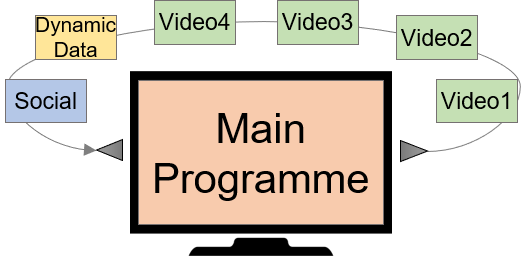
\includegraphics[width=0.5\textwidth]{uc1a.png}
		\caption{Adaptation outcome in use case 1}
		\label{fig:uc1a}
	\end{center}
\end{figure} 

The overall adaptation quality following equation \ref{Eq:E-All} is $\mathcal{E}^\mathcal{H} = 0.28$. In this context, the viewers will be able to mainly follow the TV show, while having the opportunity to perform a kind of content-hopping using the arrows in the remote control to see the other components.

It is worth noting that the adaptation value is severely affected by the inclusion of the \emph{Social} content. This is mainly due to the high interactivity it requires and the low input capabilities the Smart TV is supplied with. 

Accordingly, if the social content is not displayed, the overall quality for showing the remaining six components on TV will increase to $\mathcal{E}^\mathcal{H} =0.52$. 
On one hand, the quality of the assignment increases, since the components are more suitable on average, and on the other hand, the quality of the representation also improves, since with six components, the TV shows the components with the Split layout instead of using the Carousel layout (see Fig. \ref{fig:uc1b}).

\begin{figure}
	\begin{center}
		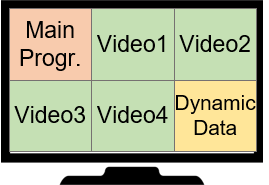
\includegraphics[width=0.25\textwidth]{uc1b.png}
		\caption{Adaptation outcome in use case 1 if the social content is not displayed}
		\label{fig:uc1b}
	\end{center}
\end{figure} 

\subsubsection{Adding a smartphone}

If a viewer is consuming the aforementioned 7 components using two devices simultaneously (a TV and a smartphone), the recommended assignation is to show the main programme and the four secondary videos on TV, while showing dynamic data and social components on the smartphone (see Figure \ref{fig:uc2a}). This scenario represents an overall quality of $\mathcal{E}^\mathcal{H}=0.66$, increasing the previous values. This mainly occurs because the components that were less suitable for the TV are now on the smartphone and also because the TV now has to represent less components, allowing a PiP layout. 

\begin{figure}
	\begin{center}
		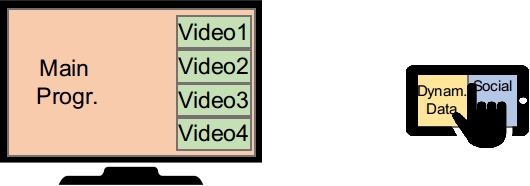
\includegraphics[width=0.5\textwidth]{ucm2a.png}
		\caption{Adaptation outcome in use case 2}
		\label{fig:uc2a}
	\end{center}
\end{figure} 

Analysing all the adaptation solutions, we found an optimal quality figure $\mathcal{E}^\mathcal{H} = 0.76$ showing the social content on the smartphone, while displaying the other components in the TV using the Split layout (see Figure \ref{fig:uc2b}).

\begin{figure}
	\begin{center}
		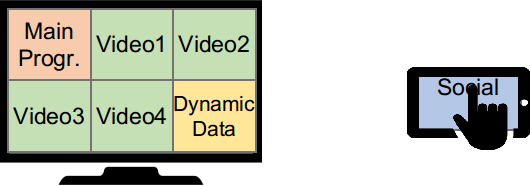
\includegraphics[width=0.5\textwidth]{ucm2b.png}
		\caption{Best possible adaptation outcome in use case 2}
		\label{fig:uc2b}
	\end{center}
\end{figure} 
In this case our two-step solution offers a quality close to 90\% ($0.66/0.76 = 0.87$) of the optimal. 

\subsubsection{Using three devices simultaneously}

If a viewer is consuming the 7 components using a TV, a laptop and a smartphone at the same time (as in Fig. \ref{fig:deployment_example}), with the properties and values specified at the beginning of this sub-section, the two-step adaptation process provides the outcome shown in Fig. \ref{fig:uc3a}.

\begin{figure}
	\begin{center}
		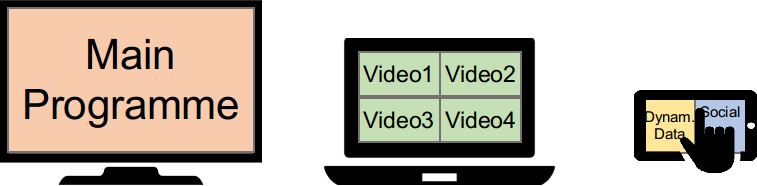
\includegraphics[width=0.6\textwidth]{ucm3a.png}
		\caption{Adaptation outcome in use case 3}
		\label{fig:uc3a}
	\end{center}
\end{figure} 

This scenario ends with an overall quality outcome of $\mathcal{E}^\mathcal{H} = 0.81$. 
It is interesting to note that with more devices, the outcome quality increases because there are components that fit (almost) perfectly to each of the devices and, with less components on each device, the quality of the representation improves. 
A discussion of how easy it is for a viewer to consume a content from several devices simultaneously could arise here. 
Thus, a parameter to penalise the use of multiple devices at the same time could be added, due to the different factors that could contribute to cognitive load, e.g., those listed in \cite{hart1988development}. 

\begin{figure}	
	\begin{center}
		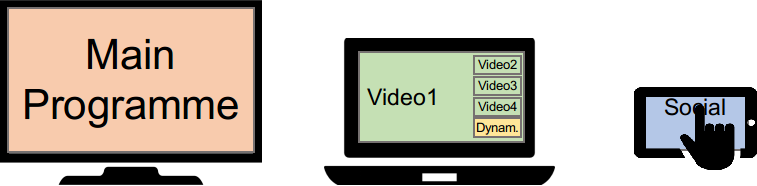
\includegraphics[width=0.6\textwidth]{ucm3b.png}
		\caption{Best possible adaptation outcome in use case 3}
		\label{fig:uc3b}
	\end{center}
\end{figure}

In use case 3, the overall optimal solution (shown in Fig. \ref{fig:uc3b}) results in a quality of $\mathcal{E}^\mathcal{H} = 0.85$.
While the optimal quality figure is marginally better than the one obtained with the two-step process, it requires evaluating ($N^{N_C}_D = 3^7 = 2187$) combinations, which is much more time and energy consuming. This was checked through an analysis of the computational efficiency of the model. 

\subsection{Evaluating the efficiency}
To analyse the computational efficiency, we ran specific performance tests using both the two-step adaptation process and the optimal solution search. 
Two scenarios have been analysed: scenario 1 considers 7 components, 3 devices, 5 properties per component, 5 properties per device, 3 layout types and 3 layout criteria; scenario 2 considers 10 components, 3 devices, 10 properties per component, 10 properties per device, 3 layout types and 6 layout criteria. 
Table \ref{tab:computational} shows the time required by each device to provide a solution to the given scenarios.

\begin{table}
	\centering
	\caption {Computational cost}\label{tab:computational}
	\begin{tabular}{||c|c|c|c||}
		\hline
		\textbf{Device} & \textbf{Tablet} & \textbf{Laptop} & \textbf{TV} \\
		\hline
		\multicolumn{4}{||c||}{\cellcolor{lightgray}\textbf{Latencies for two-step adaptation (s)} }\\
		\hline
		\textbf{Scenario 1} & 0.011 & 0.003 & 0.063  \\
		\hline
		\textbf{Scenario 2} & 0.026 & 0.006 & 0.137  \\
		\hline
		\multicolumn{4}{||c||}{\textbf{\cellcolor{lightgray} Latencies for optimal adaptation (s)} }\\
		\hline
		\textbf{Scenario 1} & 0.671 & 0.240 & 1.196  \\
		\hline
		\textbf{Scenario 2} & 9.744 & 3.179 & 28.680  \\
		\hline
		
		\hline
	\end{tabular}
\end{table}

In the first scenario, even if the two-step adaptation is much more efficient, neither method would impact the responsiveness of the user experience. However, in the second scenario, the times required to calculate the optimal solution dramatically increase, resulting in unacceptable poor responsiveness.   

As a summary of the validation of the two-step adaptation process, the experiments show that, when parameterising the proposed methodology with reasonable figures, the outcome fits adequate multi-device user interfaces, mostly coinciding with the outcome of the specific adaptation rules developed by broadcasters and researchers during the application deployment in Chapter \ref{chap:deployment} and providing a responsive (although sub-optimal) outcome efficiently. 

\subsection{Evaluating the universality of the methodology}

One of the goals of our adaptation model is to be general enough to adapt to technological evolution (e.g., forthcoming devices) and new broadcast trends or user habits, to simplify developers' work and allow for adaptive UIs on top of the adaptation system. That is why the model can be adapted, modified or oriented to other specific use cases and circumstances, while still following the proposed methodology. 
We have identified three main dimensions that could be added or modified:
\begin{itemize}
	\item UI elements (types of components, devices or layouts) and properties to adapt the model to technological and broadcasters' changes;
	\item Evaluation criteria, to adapt the model to the user;
	\item Additional context parameters that can improve the user experience. These include parameters of user context (e.g., location in the room), physical context (e.g., ambient light), and infrastructure context (e.g., saturation of device capabilities due to an excess of assigned components).
\end{itemize}


In this sub-section, different examples are provided to extend the proposed methodology and evaluate its universality.

\subsubsection{Adding a new property to the component and device types}

Consider, following the deployment performed in \cite{dominguez2017deployment}, that the \textit{Dynamic Data} component shows vote counting through a complex 3D graph type and that the \textit{Secondary Videos} have a high resolution with high decoding demands. In these cases, strong graphic capabilities would be useful. 

This will require an additional property to be considered, called \textit{Graphic/video requirements}, for the component types, having a value of $1$ for \textit{Dynamic Data}  and $0.3$ for the \textit{Secondary videos} (see Table \ref{tab:compgv}). In the same way, an additional property could be considered for the device types, called \textit{Graphic/video capabilities}, where TVs and mobile devices (both smartphones and tablets) would have a poor value (see Table \ref{tab:devgv}) and laptops would have the highest possible value. The affinity matrix will emphasise the impact of the \textit{Graphic/video requirements} with the \textit{Graphic/video capabilities} (see Table \ref{tab:affgv}).


%Tabla componentes con graphic requirements
\begin{table}
	\centering
	\caption {Components parametrisation for Graphic/video requirements} \label{tab:compgv}
	\begin{tabular}{||M{10em}|M{6cm}||}
		
		\hline \textbf{Properties} & \textbf{Graphic/video Requirements} \\
		\hline \textbf{Main} & 0 \\
		\hline \textbf{Secondary videos} & 0.3 \\
		\hline \textbf{Banner} & 0 \\
		\hline \textbf{Static data} & 0 \\
		\hline \textbf{Dynamic data} & 1 \\
		\hline \textbf{Social} & 0 \\
		\hline \textbf{UGC} & 0 \\
		\hline \textbf{Advertisement} & 0 \\
		\hline
		
	\end{tabular}
\end{table}


%Tabla devices con graphic capabilities
\begin{table}
	\centering
	\caption {Devices parametrisation for Graphic/video capabilities} \label{tab:devgv}
	\begin{tabular}{||c|c||}
		
		\hline
		\textbf{Properties} & \textbf{Graphic/video capabilities} \\
		\hline
		\textbf{Smartphone} & 0.2 \\
		\hline
		\textbf{Tablet} & 0.2 \\
		\hline
		\textbf{Laptop} & 1 \\
		\hline 
		\textbf{SmartTV} & 0 \\
		\hline
	\end{tabular}
\end{table}


%Tabla affinity con graphic requirements and capabilities
\begin{table*}
	\centering
	\caption {Affinity matrix considering Graphic/video capabilities and requirements}\label{tab:affgv}
	\begin{tabular}{||c|c|c|c|c|c|c||}
		\hline
		\textbf{} & \textbf{Scr. size} & \textbf{Inp. cap.} & \textbf{Proc. cap.} & \textbf{Priv.} & \textbf{Broad. cap.} & \textbf{G/V cap.}\\
		\hline
		\textbf{Attention} & 1 & 0 & 0 & 0.1 & 0 & 0\\
		\hline
		\textbf{Interactivity} & 0.1 & 1 & 0.5 & 0.9 & 0 & 0\\
		\hline
		\textbf{Processing req.} & 0.3 & 0.3 & 1 & 0 & 0 & 0  \\
		\hline
		\textbf{Broadcast req.} & 0 & 0 & 0 & 0 & 1 & 0 \\
		\hline 
		\textbf{Confidentiality} & 0 & 0 & 0 & 1 & 0 & 0\\
		\hline
		\textbf{Graphic/video req.} & 0 & 0 & 0 & 0 & 0 & 1 \\
		\hline
	\end{tabular}
\end{table*}

With the aforementioned novel scenario, if we replicate the environment provided by \textit{use case 3}, the outcome of the two-step adaptation shown in Figure \ref{fig:uc3b}, which is the optimal solution, is obtained instead of the previous one (shown in Figure \ref{fig:uc3a}), with a quality $\mathcal{E}^\mathcal{H} = 0.85$. 

\subsubsection{Adding a new criterion for user interface layouts}

Apart from the aforementioned visual criteria to select the best user interface layout in each case (recall that Table~\ref{tab:aparea} and Table~\ref{tab:layoutparam} were constrained to parameters related to the screen area), a broadcaster or content provider may want to consider the intrinsic interactivity required by the layout itself. 
For instance, a carousel layout requires the interaction of the viewer to spin the components of the carousel and select the one to be seen in fullscreen.
This interaction will be the most difficult with the remote control of a TV, while easiest with a trackpad on a laptop or a touch-screen device.
In the same way, PiP layouts could benefit from this interaction facilities.
Regarding the Split layout, however, the interaction is not a relevant parameter according to the opinion of broadcast professionals and researchers that participated in the deployment described in Chapter \ref{chap:deployment}. 
To take these aspects into consideration a fourth criteria $\alpha_4$ has been considered, named \textit{Interactivity compliance} and defined as the degree in which a layout is manageable in terms of interaction when it is displayed in a specific device.  

For the calculation of the aforementioned criteria, an additional layout parameter has been added to those defined in Table~\ref{tab:layoutparam}, named \textit{Interactivity requirements} (Ir) and defined as the level of interaction required by the layout to be managed by the user. Table \ref{tab:layoutir} shows the values given to Ir for each layout. 

\begin{table}
	\centering
	\caption {Input requirements for each layout}\label{tab:layoutir}
	\begin{tabular}{||c|c|c|c||}
		\hline
		\textbf{Parameter} & \textbf{PiP} & \textbf{Split}  & \textbf{Carousel} \\
		
		\hline
		\textbf{Ir}  & 0.4 & 0 & 0.4\\
		\hline
	\end{tabular}
\end{table}

Furthermore, an additional dimension has been added to the parameters related to each device (see Table \ref{tab:aparea}) that are considered to calculate the quality of a layout. 
In this case the new parameter has been the \textit{Input capabilities} (Ic) of each device. Table \ref{tab:devic} shows the values given to Ic for each device.

\begin{table}
	\centering
	\caption {Input capabilities per device}\label{tab:devic}
	\begin{tabular}{||c|c|c|c|c||}
		\hline
		\textbf{Device} & \textbf{Smartphone} & \textbf{Tablet} & \textbf{Laptop} & \textbf{SmartTV}\\
		
		\hline
		\textbf{Input cap. (Ic)} & 0.7 & 0.8 & 1 & 0.3\\
		\hline
	\end{tabular}
\end{table}


Figure \ref{fig:qualIntCrit} shows the representation of the quality of the layouts in terms of the number of components for Smart TV devices, after adding the criteria of interaction of the layouts. Again, this representation follows Eq. \ref{Eq:layoutq}, with $k \in [1,4]$ and using $w_1=1.4$, $w_2=0.3$, $w_3=1.2$ and $w_4=1$ as the weights for each criterion, where $w_4$ denotes the weight assigned to the new interaction criteria.

\begin{figure}
	\begin{center}
		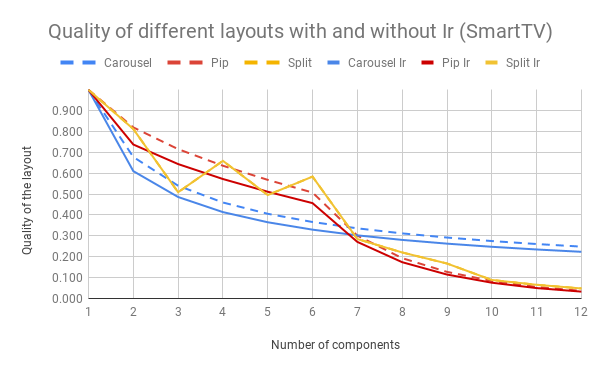
\includegraphics[width=0.8\textwidth]{graphs2_crop.png}
		\caption{Quality of the layouts in terms of number of components with interaction criteria (straight line) and without (dashed).}
		\label{fig:qualIntCrit}
	\end{center}
\end{figure}

As shown in Figure \ref{fig:qualIntCrit}, the quality of the layouts changes when using the interaction compliance criteria: the quality decreases for both the Carousel and PiP layouts, reinforcing Split as the best layout.

Other user interface layouts criteria could also be considered, such as the prioritisation of a specific component in comparison with the other components represented on the same screen. For example, the Split layouts seem to harmonise the priority of all the components shown in the display, even though the position itself could be a way to prioritise. However, in the PiP layout, the predominance of a component over the other seems to be much clear. A reasonable criterion could improve the quality of the PiP layout for a device that contains the main programme (such as the TV), while promoting a more equitable layout, such as Split, for a device that shows some secondary videos (such as a laptop).

As a summary, this subsection shows that the proposed methodology is general, flexible and adaptable to any kind of multi-device media service. The model will not change depending on the use case, it just needs to be fine-tuned by adding or modifying parameters.

\section{Conclusions}
This chapter proposes a methodology for multi-device user interface adaptation in media services, such as a hybrid broadcast-broadband TV programme. The definition of this methodology provides a general adaptation model as an outcome, which identifies and characterises all the elements of the user interface, analyses the role of the context, and provides an approach to address the challenge of dividing the process into two different sub-processes to make it responsive.

The aforementioned research has allowed the model to be formally described and provides a comprehensive example of how an implementation could be performed. Reasonable parameters have been used for this, which provide an outcome that coincides with the output of the adaptation rules developed by the broadcasters and researchers during the application deployment described in Chapter \ref{chap:deployment} and published in \cite{dominguez2017deployment}. Moreover, the model quality, efficiency and universality have been validated and the following conclusions have been drawn:
\begin{itemize}
	\item Suboptimal solutions obtained by the two-step adaptation process are reasonably good and meet the expectations of broadcasters and researchers. In the use cases tested  they offer a quality of approximately 90\% of the optimal. 
	\item The two-step adaptation process is much more efficient than the search of the global optimal solution in terms of the processing time and hence of the power consumption.
	Responsiveness and low latencies are guaranteed through two sequential steps, but not through the exploration of the problem as a whole.
	\item  The developed model is general enough to be extended to any type of content, device, context or evaluation criteria and ready for technological changes as well as continuous adaptive learning processes. 
\end{itemize}